\chapter{Моделювання та ідентифікація фізичної системи пов'язаних релаксаційних генераторів}

\newcommand{\RelaxBjtIi}{системи з трьох пов'язаних релаксаційних генераторів на парі компліментарних транзисторів}
\newcommand{\RelaxShIi}{системи з трьох пов'язаних релаксаційних генераторів на основі тригерів Шмідта}

\section{Релаксаційні генератори: застосування і моделі}

Релаксаційні генератори, прямо або побічно, набули широкого
поширення в схемотехніці. В першу чергу --- як генератори
сигналів, в першу чергу пилкоподібної форми~\cite{horowitz,
mishenko_du_small_relax}. Деякі підсистеми електричних схем, хоч і
не належать безпосередньо до релаксаційних генераторів,
проявляють схожу динаміку. В першу чергу це імпульсні системи
живлення, такі як сучасні блоки живлення електронної техніки,
DC/DC перетворювачі, системи позиціювання~\cite{atu_st104b}.

Основними компонентами релаксаційного генератора
(рис.~\ref{atu:f:relax_types}) є накопичувальний елемент, найчастіше
конденсатор C, ланцюги заряду і розряду (в загальному випадку
нелінійні), представлені на умовній схемі позначеннями
$ R \Tidx{ch} $ і
$ R \Tidx{dis} $ відповідно, і нелінійний (гістерезисний)
елемент (CTRL), що перемикає генератор з режиму зарядки в режим
розрядки і навпаки. Як такий елемент може використовуватися
динистор, газорозрядна лампа, тригер Шмідта, інші електронні елементи.

\begin{figure}[htb!]
  \centerline{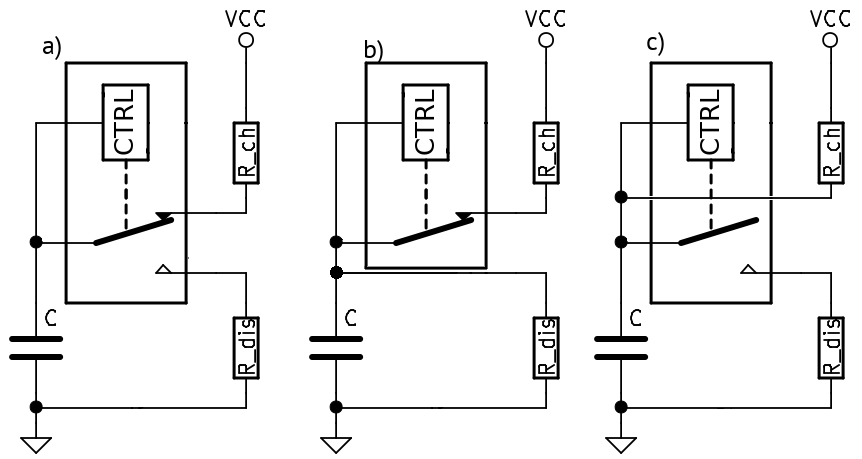
\includegraphics[width=0.8\textwidth]{p/relax_types.png} }
\caption{Умовні схеми релаксаційних генераторів.}
\label{atu:f:relax_types}
\end{figure}

Представлені на рис.~\ref{atu:f:relax_types} основні види релаксаційних
генераторів відрізняються тим, як перемикаючий елемент
(CTRL) підключає ланцюга заряду і розряду. У схемі (a)
одночасно підключено тільки один з цих ланцюгів. Таке
схемотехнічне рішення використовується досить рідко. Схема (b)
характеризується тим, що ланцюг розряду підключено постійно,
а ланцюг розряду включаться при досягненні певного умови. Таке
підключення характерно для схем імпульсних перетворювачів і
стабілізаторів напруги. У схемі (c) навпаки, процес заряду
відбувається постійно, а розряд --- за умови заданому
елементом, що перемикає. Таке включення характерно для
генераторів пилкоподібних та інших сигналів. У даній роботі в
основному будуть розглянуті системи і їх моделі, засновані на
схемі (с). Принципової різниці при використанні і моделюванні
інших подібних схем не спостерігається. Існують і інші схеми,
що використовують принцип роботи релаксаційного генератора,
наприклад мультивібратори, але дослідження їх моделей виходить
за рамки даної роботи.



Основними параметрами схем з релаксаційним генераторами є
напруги включення
$ V \Tidx{on} $ і виключення
$ V \Tidx{off} $ елемента, що перемикає (CTRL), напруга живлення
$ V \Tidx{cc} $, ємність конденсатора
$ C $, опори ланцюгів зарядки
$ R \Tidx{ch} $ і розрядки
$ R \Tidx{dis} $. У даній роботі, для кращого прояву хаотичних
режимів, будемо вважати, що часи зарядки і розрядки істотно
відрізняються~\cite{atu_asau19}. Не знижуючи спільності, вважаємо, що
$ R \Tidx{ch} \gg R \Tidx{dis} $. При попередньому аналізі можна вважати
$ R \Tidx{dis} = 0 $. Проте, для забезпечення коректності чисельного
моделювання, а також забезпечення адекватності моделі потрібне
застосування ненульового значення
$ R \Tidx{dis} $. Змінними стану є напруга на конденсаторі
$ V \Tidx{c} $ і стан елемента, що перемикає
$ \mathrm{On}()$. У разі використання декількох релаксаційних
генераторів ці величини будемо позначати відповідно як
$ V_{i} $ і
$ \mathrm{On}_{i}() $. При цьому
$ \mathrm{On}_{i}(V \Tidx{c}, \ldots) $ --- релейний гістерезисний елемент, що
має пам'ять і задається алгоритмічно.

У цих умовах приймемо для визначеності (а в більшості
схемотехнічних реалізацій це так і є), що ланцюг зарядки включено
постійно, а ланцюг розрядки включається при
$ V \Tidx{c}> V \Tidx{on} $ і вимикається при
$ V \Tidx{c} <V \Tidx{off} $.

З урахуванням цих позначень динаміка релаксаційного релаксаційного
генератора визначається наступним чином:
%
\begin{equation}
  C \od{V_c}{t}
  =
  \frac{V\Tidx{cc} - V\Tidx{c}}{R\Tidx{ch}}
  - \frac{V\Tidx{c}}{R\Tidx{dis}} \cdot \mathrm{On}().
  \label{atu:eq:relax0}
\end{equation}

У разі одного релаксаційного генератора рівняння (\ref{atu:eq:relax0})
можна привести до безрозмірного вигляду, використовуючи набір
очевидних перетворень. В першу чергу, величина
$ C R \Tidx{ch} $ визначає постійну часу процесу заряду, а процес
розряду за умови
$ R \Tidx{ch} \gg R \Tidx{dis} $ будемо вважати, що відбувається практично
миттєво. Позначимо:
%
\begin{equation}
  t_u = \frac{t}{R\Tidx{dis} C} .
  \label{atu:eq:t_u_relax}
\end{equation}

Далі, так як напруга не опускається нижче
$ V \Tidx{off} $, то має сенс прийняти це значення як нульовий потенціал,
з відповідним коригуванням залишилися величин. При подальшому
приведенні напруг до безрозмірного вигляду можна зробити двома
способами: прийняти за одиницю або скориговану напругу живлення
$ V \Tidx{cc} -V \Tidx{off} $, або ж скориговану напругу включення
$ V \Tidx{on} -V \Tidx{off} $. Для одного релаксаційного генератора вибір
способу практично ні на що не впливає, але при використанні
декількох --- зручнішим стає перший спосіб. Таким чином,
позначимо:
%
\begin{equation}
  v(t) = \frac{V(t)-V\Tidx{off}}{V\Tidx{cc}-V\Tidx{off}},
  \quad
  v\Tidx{on} = \frac{V\Tidx{on}-V\Tidx{off}}{V\Tidx{cc}-V\Tidx{off}},
  \quad
  v\Tidx{on} \in ( 0; 1 ).
  \label{atu:eq:v_u_relax}
\end{equation}

З урахуванням цих позначень, рівняння, що описує процес однієї
зарядки набуває вигляду:
%
\begin{equation}
  \od{v}{t_u} = 1 - v( t_u ),
  \quad
  v( t_u ) < v\Tidx{on},
  \quad
  v(0) = 0.
  \label{atu:eq:relax_charge_u}
\end{equation}

Рішенням (\ref{atu:eq:relax_charge_u}) є
%
\begin{equation}
  v(t_u) = 1 - \exp( - t_u ) ,
  \quad
  v( t_u ) < v\Tidx{on}.
  \label{atu:eq:relax_charge_u_solu}
\end{equation}

Безрозмірний час перемикання
$ T_u $, при нехтуванні часом розрядки, визначає безрозмірний
період:
%
\begin{equation}
  v\Tidx{on} = 1 - \exp( - T_u ),
  \quad
  T_u = - \ln ( 1 - v\Tidx{on} ).
  \label{atu:eq:T_u_relax}
\end{equation}

Таким чином, в лінійному наближенні, і зневажаючи часом
розрядки, поведінка системи визначається одним безрозмірним
параметром
$ v \Tidx{on} $, і визначає інший безрозмірний параметр
$ T_u $. При
$ v \Tidx{on} \ll 1 $ процес зарядки є практично лінійним, усереднене значення
$ v (t_u) $:
%
\begin{equation}
  \overline{v(t_u)} =
  \frac{1}{T_u}\int\limits_{0}^{T_u} \mathrm{d}t_u
  \approx
  \frac{v\Tidx{on}}{ 2 }.
  \label{atu:eq:av_lin_relax}
\end{equation}
%
та
%
\begin{equation}
  T_u
  \approx
  v\Tidx{on}.
  \label{atu:eq:T_u_lin_relax}
\end{equation}

З іншого боку, при
$ v \Tidx{on} \to 1 $,
$ T_u \to \infty $,
та
$ \overline{v(t_u)} \to v\Tidx{on}$.

З цих спостережень зроблено висновок, що якщо для одиночного
релаксаційного генератора є можливість спостерігати період
(або ж частоту) коливань, то безрозмірний параметр
$ v \Tidx{on} $ визначається просто і без істотних похибок
вимірювання. І навпаки, якщо для вимірювання доступна величина
$ \overline{v (t_u)} $, то при малих значеннях
$ v \Tidx{on} $ складнощів при вимірюванні (або ж ідентифікації) немає,
а при
$ v \Tidx{on} \approx 1 $ малі зміни
$ \overline{v (t_u)} $ призводять до практично не обмежених змін
$ t_u $, що не сприяє процесу ідентифікації.

Проте, в разі, коли в одному генераторі використовується
кілька релаксаційних елементів, то поняття періоду не має
особливого сенсу, або ж взагалі не визначено в разі хаотичної
поведінки. Тому, вимірювання усереднених напруг може виявитися
практично єдиним способом оцінки параметрів системи.


Якщо ж застосовується в одній схемі кілька релаксаційних
генераторів з різними параметрами, або ж розглядаються
нелінійні залежності струмів від різниць потенціалів, то
приведення до безрозмірного вигляду практичного сенсу не має,
однак закономірності, отримані для простого випадку, корисні
для аналізу можливих критеріїв ідентифікації.


У попередньому аналізі було прийнято
$ V\Tidx{cc} = \mathrm{const} $. Однак, при аналізі динаміки реальних
генераторів моделі, що використовують це припущення, не цілком
адекватно описують динаміку, так як реальні джерела напруги
мають обмежені можливості. При описі одного релаксаційного
елемента обмеженість можливостей джерела елементарно
компенсується додаванням внутрішнього опору джерела до
$ R \Tidx{dis} $. У разі, коли одне реальне джерело живить множину
генераторів, такий підхід стає непридатним. В цьому випадку,
для збереження умови
$ V \Tidx{cc} = \mathrm{const} $ вважатимемо, що ця величина описує ЕРС джерела
без навантаження, а всі релаксаційні генератори отримують від
шини живлення з напругою
$ V_b (t) $, яке визначається як сумарним струмом споживання,
так і обмеженим можливостями шини живлення, які, в першому
наближенні, описуються ефективним опором
$ R_b $, який визначається як внутрішнім опором джерела, так і
опором самої шини, тобто
%
\begin{equation}
  V_b(t) = V\Tidx{cc} - R_b \sum\limits_{i=0}^{n-1} I_i(t),
  \label{atu:eq:V_b_relax}
\end{equation}
%
де $i$ ---
порядковий номер релаксаційного елемента,
$ I_i (t) $ --- струм, який він споживає.


\section{Властивості і моделі елемента, що перемикає на парі біполярних транзисторів}
\label{atu:sec:relax3d_sw}

Як вже було зазначено, для реалізації
елемента, що перемикає, існує широкий спектр
можливостей. Проте, в рамках даної роботи не ставляться завдання
ні аналізу роботи якогось певного елемента, ані огляду всіх
існуючих. Оскільки основним завданням даного розділу є синтез
системи ідентифікації для реального генератора, а також аналіз
можливості цієї системи, то в якості перемикаючих елементів
релаксаційних генераторів має сенс вибирати ті, властивості
яких дозволяють як з мінімальними зусиллями, так і мінімальними
перешкодами сполучати досліджуваний генератор з вимірювальної
системою, реалізованої на основі мікроконтролера. Отже, з
розгляду виключено газорозрядні лампи, динистори, і подібні
елементи, що вимагають високої напруги живлення.


Одним з можливих способів реалізації
елемента, що перемикає, є схема з двох комплементарних біполярних
транзисторів, яка була застосована A.S.~Elwakil і M.P.~Kennedy~\cite{kennedy1999} для
створення низьковольтного, малопотужного хаотичного
генератора. Розглянута в згаданій роботі схема хаотичного
генератора вельми цікава, але включає індуктивний елемент,
що ускладнює створення точних, і в той же час простих
моделей через складні гістерезисні
явища в феромагнітному осерді. При цьому відносно високий
частотний діапазон ускладнює процес вимірювання. Тому,
в даному дослідженні з цієї роботи буде використовуватися
тільки елемент, що перемикає,~(рис.~\ref{atu:f:relax3d_switch}).

\begin{figure}[htb!]
  \centerline{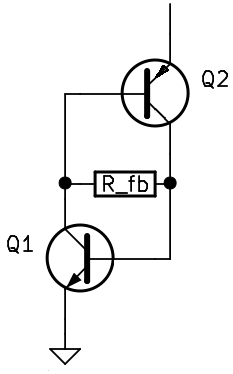
\includegraphics[width=0.25\textwidth]{p/relax3d_switch.png} }
\caption{Схема елемента, що перемикає, на компліментарних біполярних транзисторах}
\label{atu:f:relax3d_switch}
\end{figure}



Результати чисельного моделювання роботи даної схеми, отримані
за допомогою програми моделювання ``ngspice'' 26 представлені на
рис.~\ref{atu:f:relax3d_sw_vah}. Початкова схема була розширена керованим
джерелом живлення і опором навантаження
$ R_n $. Це дозволило отримати сімейство вольт-амперних
характеристик при різних значеннях
$ R_{fb} $.

\begin{figure}[htb!]
  \centerline{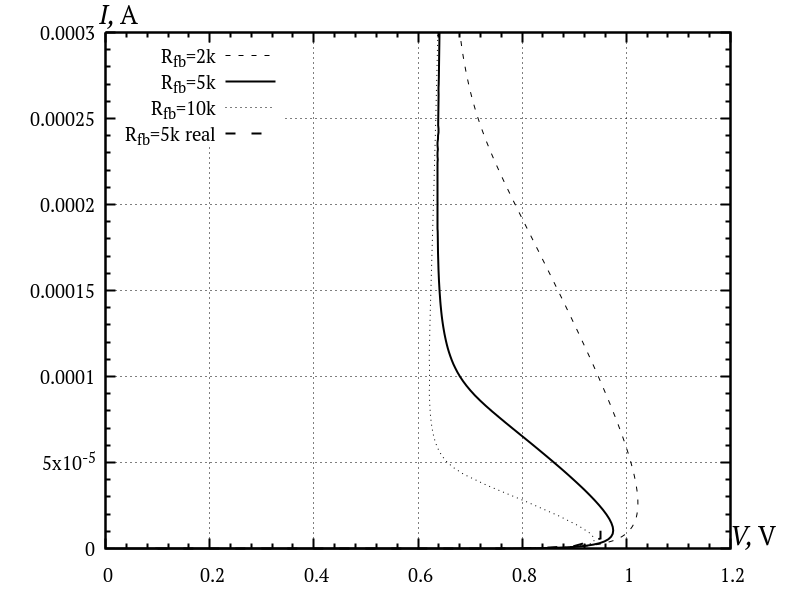
\includegraphics[width=0.6\textwidth]{p/relax3d_sw_va.png} }
\caption{Сімейство розрахункових вольт-амперних характеристик
елемента, що перемикає, на компліментарних біполярних
транзисторах, в порівнянні з реальними даними}
\label{atu:f:relax3d_sw_vah}
\end{figure}


Все вольт-амперні характеристики, отримані шляхом моделювання,
мають S-подібну форму, характерну для бістабільних
елементів, таких як динистори, газорозрядні лампи і т.д. Ділянки
характеристик, відповідні до від'ємного диференціального
опору, є нестійкими, і в реальних схемах не реалізуються. Тому
реальні дані для цих ділянок не представлені. Те, що ці значення
були отримані в програмі моделювання, свідчить про недостатню
адекватність застосовуваних моделей. Ще одним підтвердженням
обмеженою адекватності моделей, що використовуються в
програмах для моделювання, заснованих на ``spice'', є той факт, що
в розглянутих програмах з цього сімейства не вдалося досягти
працездатності моделі релаксаційного генератора із зазначеним
елементом, що перемикає.


Складна нелінійна вольт-амперна характеристика розглянутого
елемента, що перемикає, тим не менш, в широкому діапазоні
параметрів, не служить серйозною перешкодою для
моделювання релаксаційного генератора в цілому. Як випливає
з представлених графіків, струм до моменту перемикання не
перевищує
$ \SI{2 e-6}{\ampere} $, а на значній частині робочої ділянки не перевищує
$ \SI{1e-8}{\ampere} $, що для багатьох (але не для всіх) умов може
розглядатися як просто вимкнений стан,
$ I \Tidx{dis} = 0 $.

З іншого боку, після перемикання ефективний опір цього елемента досить малий,
$ R \Tidx{dis} \approx \SI{20}{\ohm} $, що для аналітичної оцінки практично
еквівалентно миттєвому розряду, а для чисельного моделювання
як похибки у визначенні
$ R \Tidx{dis} $ практично на порядок, так і нелінійна залежність
істотної ролі не грають. Тому, при використовуваних діапазонах
параметрів, для моделювання даний елемент можна представити
у вигляді функції
$ \mathrm{On} (V) $. Параметри цієї функції ---
$ V \Tidx{on} $ і
$ V \Tidx{off} $ можна визначити експериментально. Експериментально
отримана залежність для
$ V \Tidx{on} (R_{fb}) $ представлена на (рис.~\ref{atu:f:relax3d_bjt_v_onn}), а
величина
$ V \Tidx{off} $ виявилася практично не залежною від
$ R_{fb} $.

\begin{figure}[htb!]
  \centerline{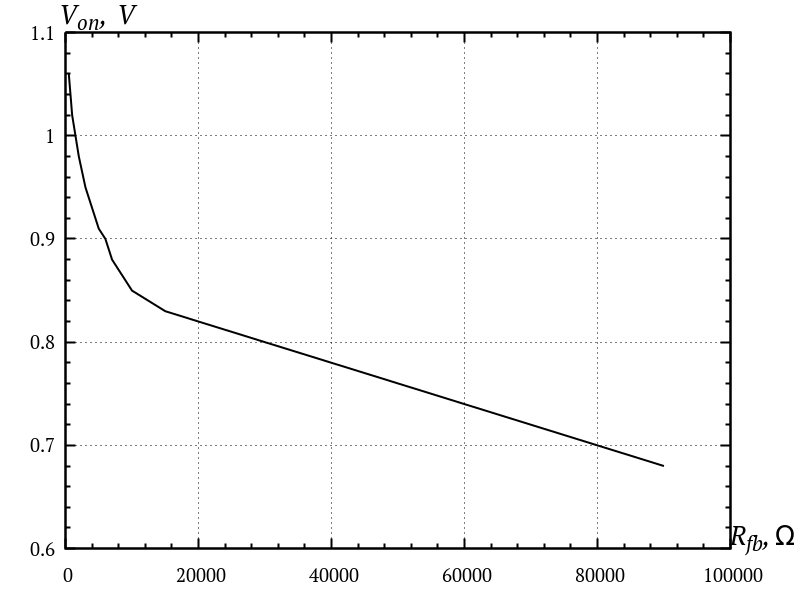
\includegraphics[width=0.7\textwidth]{p/r_fb-V_on.png} }
\caption{Експериментальна залежність $ V \Tidx{on} (R_{fb}) $ для елемента, що перемикає на двох комплементарних біполярних транзисторах}
\label{atu:f:relax3d_bjt_v_onn}
\end{figure}

Як і для багатьох електронних схем, які використовують
властивості p-n переходів, для даної схеми характерна сильна,
практично експоненціальна залежність струму від температури. У
даній роботі при проведенні експериментів розкид температури
не перевищував
$ \SI{5}{\kelvin} $, що дозволило уникнути зайвого ускладнення моделі.


Слід зазначити і певну обмеження при використанні простої
$ \mathrm{On}{v} $ моделі елемента, що перемикає. Для пояснення
причини цього обмеження розглянемо ділянки вольт-амперних
характеристик, що безпосередньо передують переключенню
(рис.~\ref{atu:f:relax3d_sw_vah_mini}).

\begin{figure}[htb!]
  \centerline{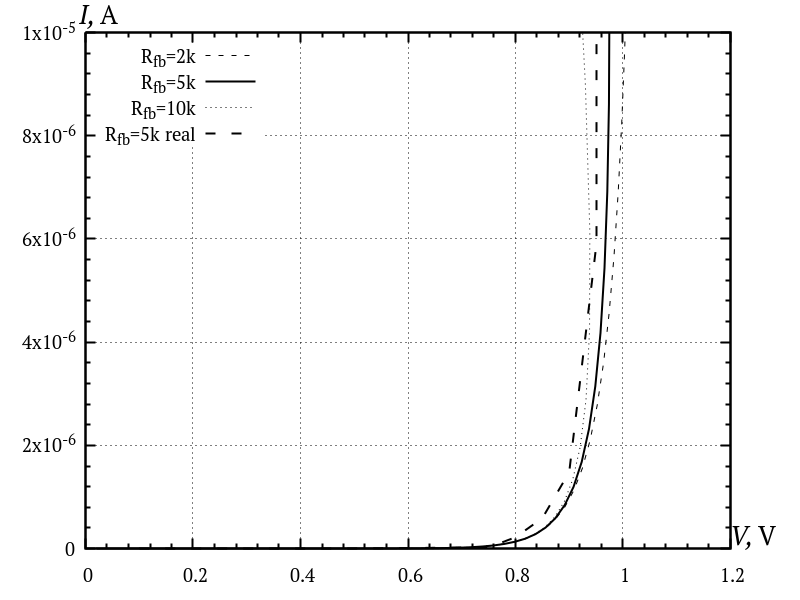
\includegraphics[width=0.6\textwidth]{p/relax3d_sw_va_mini.png} }
\caption{Ділянки вольт-амперних характеристик елемента, що перемикає, що безпосередньо передують переключенню}
\label{atu:f:relax3d_sw_vah_mini}
\end{figure}

У цих умовах графіки схожі на характеристики елементів або
ж схем, призначених для стабілізації напруги, тобто у цих
умовах суттєві зміни струму відповідають малим змінам падіння
напруги. Якщо в схемі релаксаційного генератора опір
$ R \Tidx{ch} $ буде настільки великим, що струм не перевищить
максимального струму ``стабілізації'', то напруга
$ V \Tidx{on} $ ніколи не буде досягнута, і генерації коливань не
буде. Більш того, при наближенні до цього режиму адекватність
моделі буде все більш сумнівною. Один із способів протистояння
погіршення адекватності полягає в обліку істотно нелінійної
залежності струму витоку. Однак, як показали результати
моделювання, поліпшення адекватності хоч і спостерігаються,
але застосовувати таке ускладнення моделі має сенс тільки в
досить вузькому діапазоні параметрів, що не робить істотного
впливу на досягнення основних цілей даної роботи.

Таким чином, релаксаційний генератор з  елементом, що перемикає
на парі компліментарних біполярних транзисторів може
використовуватися при побудові системи пов'язаних генераторів,
а його поведінка може бути описано досить простою моделлю в
широкому діапазоні параметрів.



\section{Система з трьох пов'язаних релаксаційних генераторів на парі компліментарних транзисторів}
\label{atu:sec:relax3d}


Пропонований хаотичний генератор являє собою систему з трьох
релаксаційних генераторів, елемент, що перемикає в кожному з
них реалізований на парі компліментарних транзисторів~\cite{atu_st107}
(рис.~\ref{atu:f:relax3d_schem}).

\begin{figure}[htb!]
  \centerline{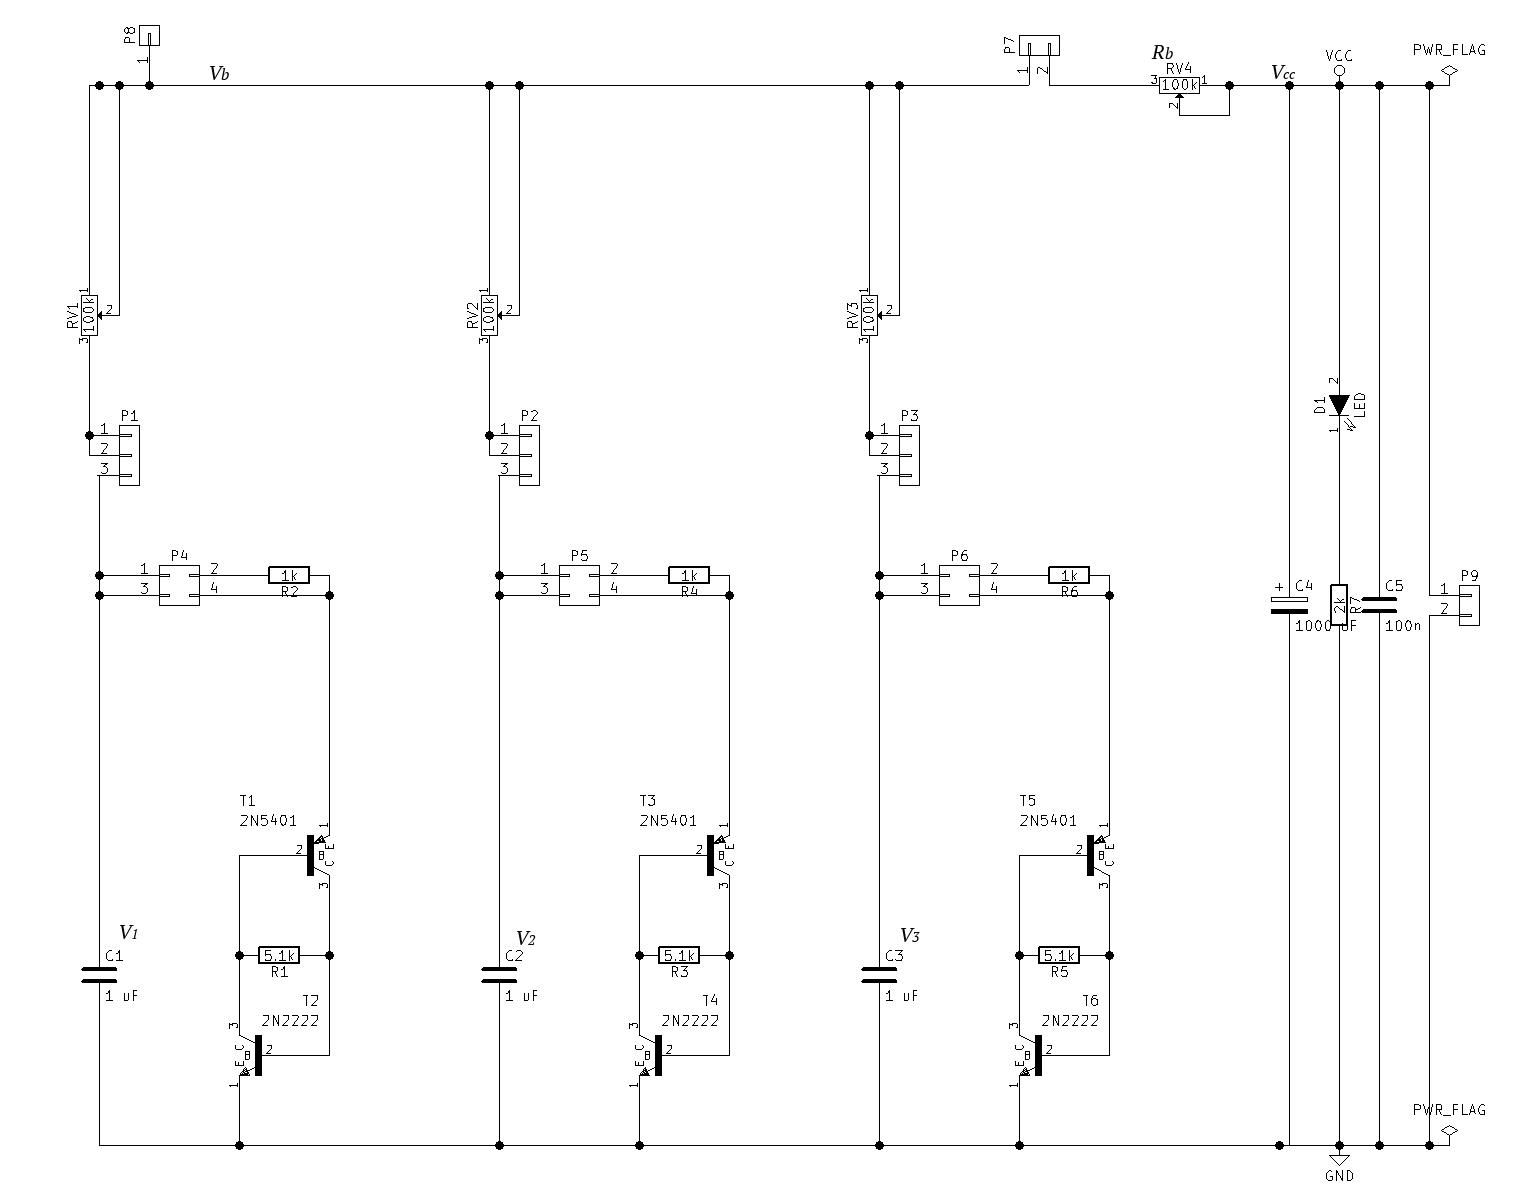
\includegraphics[width=0.96\textwidth]{p/relax3d_schem.png} }
\caption{Електрична схема \RelaxBjtIi}
\label{atu:f:relax3d_schem}
\end{figure}

При створенні даної схеми переслідувалися наступні завдання:
\begin{itemize}


  \item
    працездатність схеми при малої напрузі живлення
    $ V \Tidx{cc} $, бажана можливість використання загального живлення
    з мікроконтролером --- при цьому не потрібні додаткові
    елементи погоджування між генератором і АЦП мікроконтролера
    --- отже, менше елементів, які можуть вносити спотворення при
    вимірюванні;

  \item
    відносно низькі робочі частоти релаксаційних генераторів ---
    для зменшення впливу індуктивностей і взаємних зв'язків, які
    не описуються моделлю, зменшення шумів вимірювання, викликаних
    спотвореннями високочастотних сигналів;

  \item
    можливість оперативно змінювати параметри схеми, як відключаючи
    окремі генератори, так і вводячи додаткові елементи.

\end{itemize}

Зовнішній вигляд зібраної електричної схеми на макетної платі
представлений на рис.~\ref{atu:f:relax3d_board}.

\begin{figure}[htb!]
  \centerline{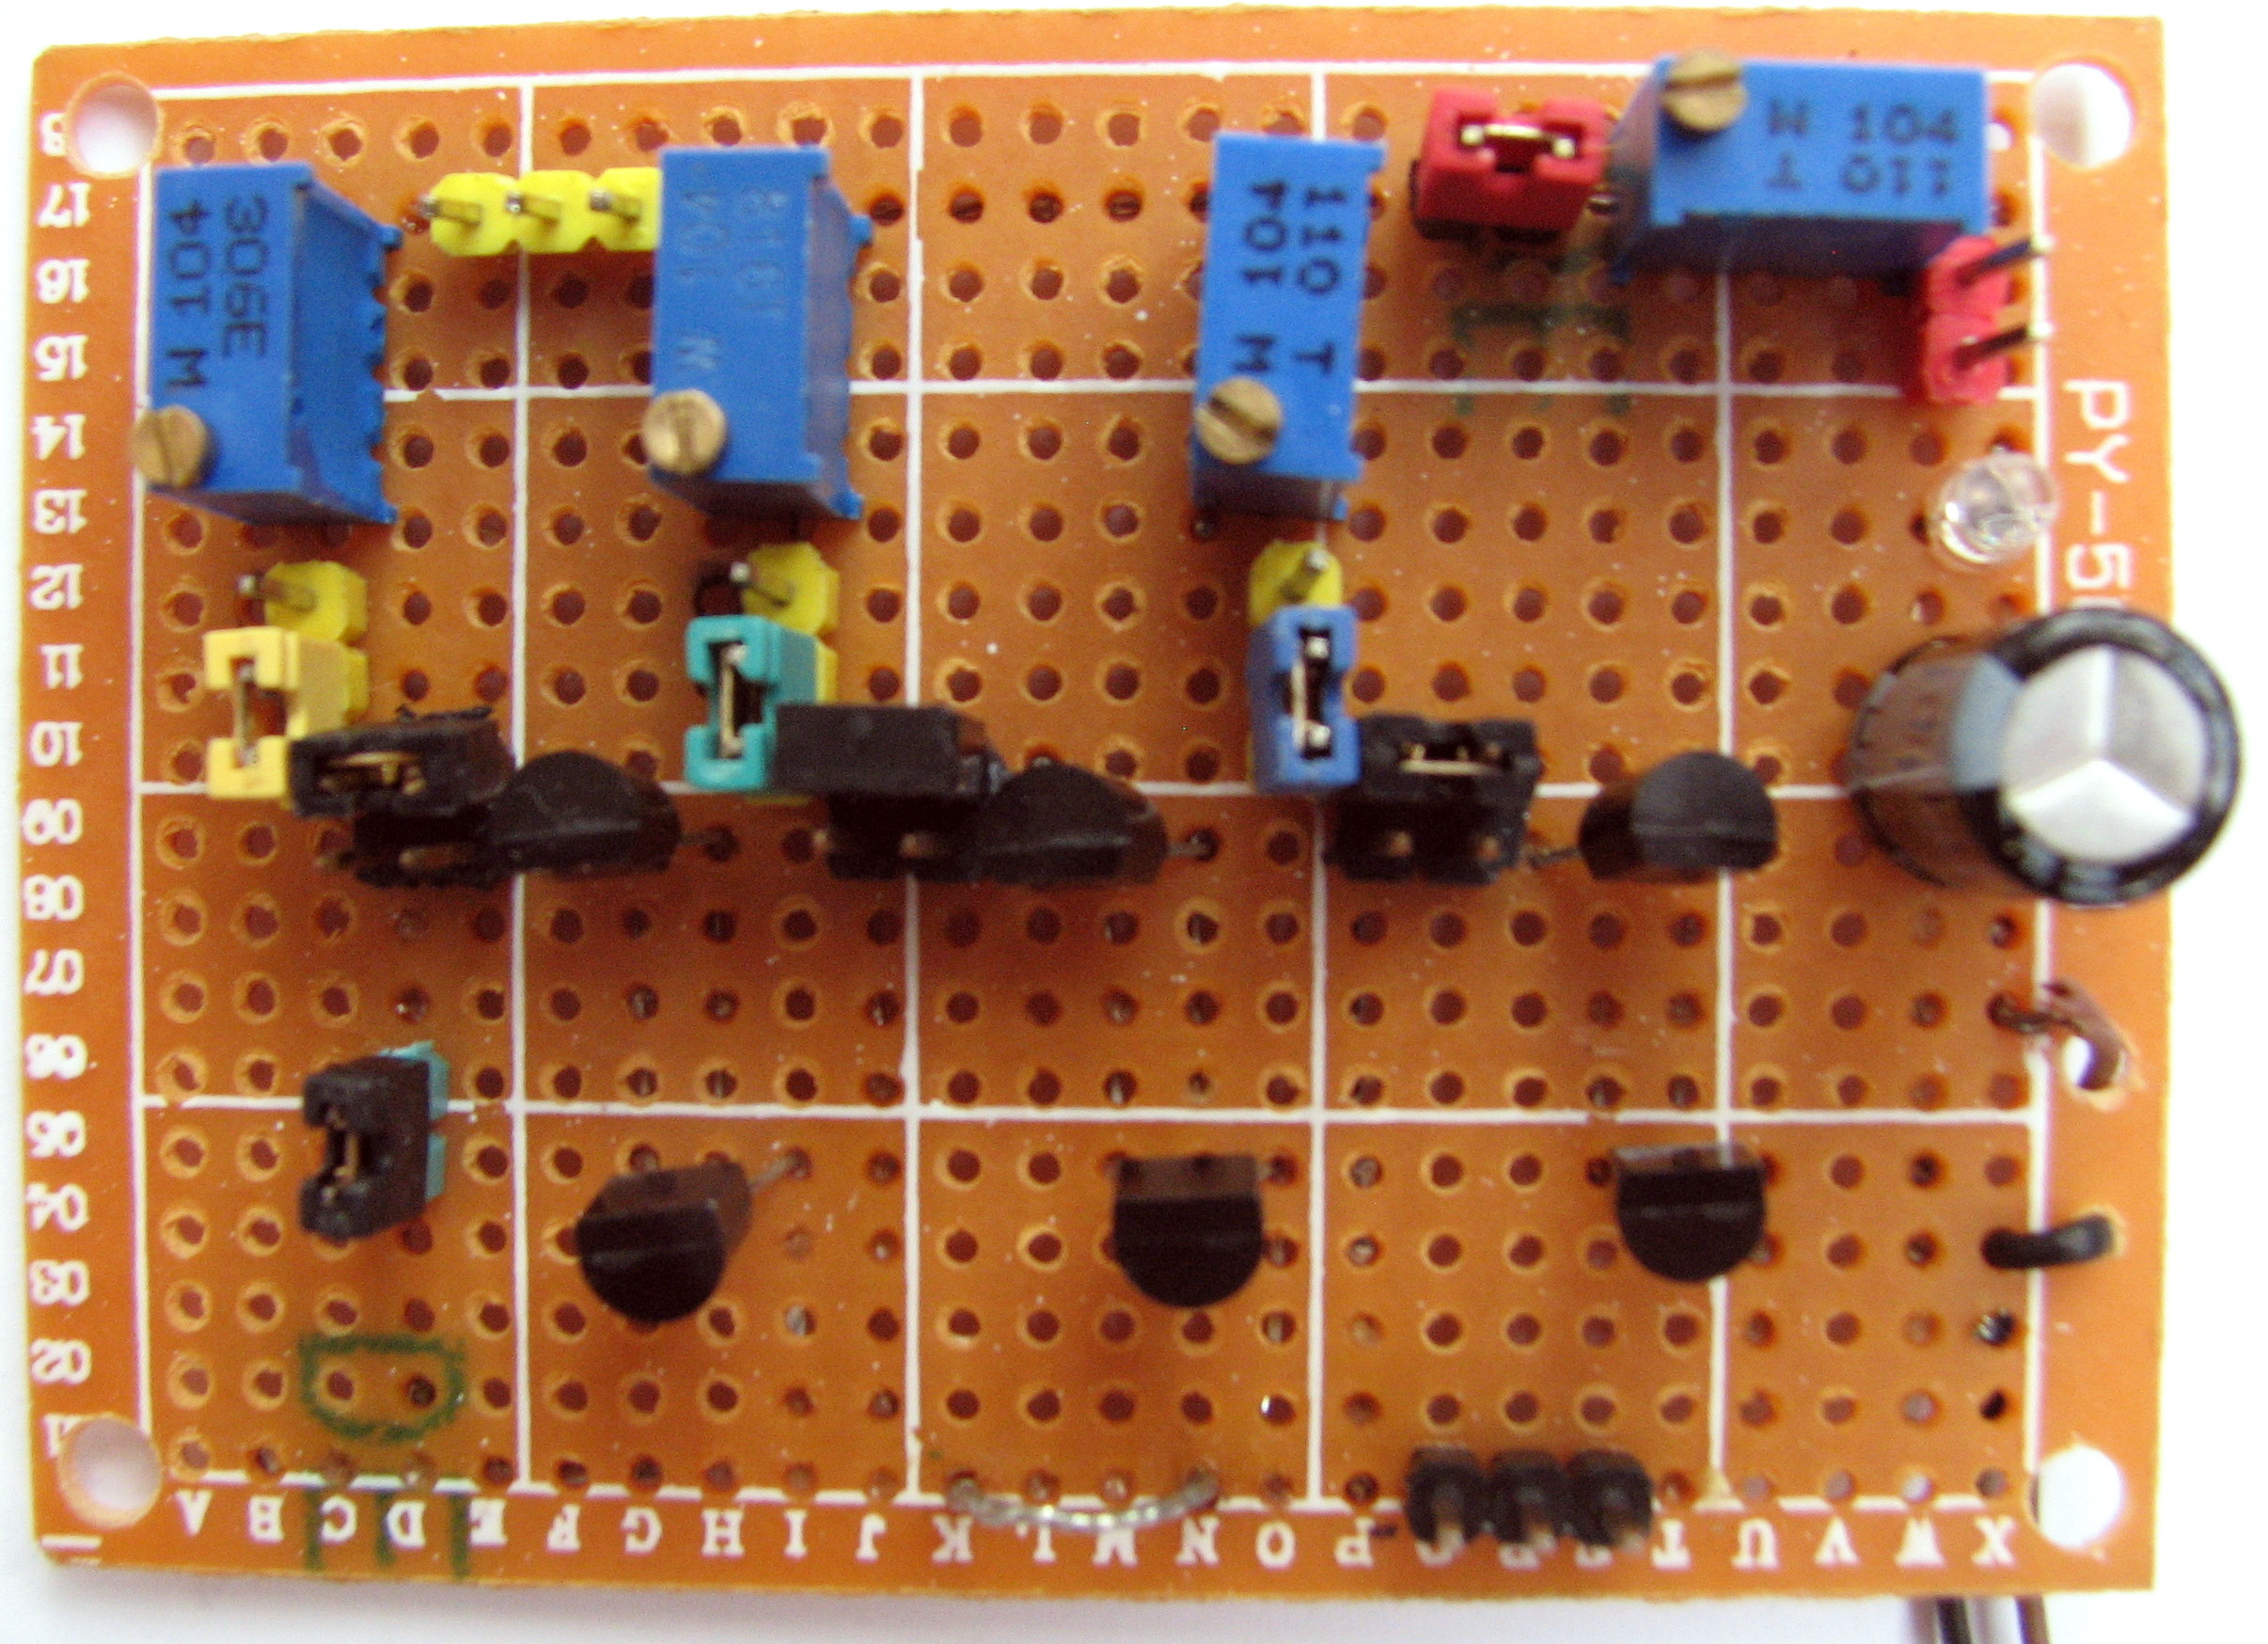
\includegraphics[width=0.6\textwidth]{p/relax3d_board.jpg} }
\caption{Схема (рис.~\ref{atu:f:relax3d_schem}), зібрана на макетної платі}
\label{atu:f:relax3d_board}
\end{figure}

Дану схемотехнічну реалізацію в подальшому будемо позначати
як ``relax3d''.


Можливість роботи при низькій напрузі живлення в даній
схемі забезпечується застосуванням елемента, що перемикає
з параметрами
$ V \Tidx{on} \approx \SI{1.0}{\volt} $,
$ V \Tidx{off} \approx \SI{0.6}{ \volt} $. При цьому, напруга живлення
$ V \Tidx{cc} \approx \SI{3}{\volt} $ забезпечує достатній діапазон для зміни
параметрів генератора. Будь-яка з вимірюваних напруг
$ V_b $,
$ V_1 $ ---
$ V_3 $ ніколи не перевершує
$ V \Tidx{cc} $, що дозволяє використовувати безпосередній зв'язок між
елементами схеми і АЦП мікроконтролера. Вхідной опір каналів АЦП
$ R \Tidx{measure} \approx \SI{10e7}{\ohm} $ і ємність
$ C \Tidx{measure} \approx \SI{10}{\pico \farad} $ не вносять помітних спотворень в
роботу генератора.

Щодо низькі (десятки і сотні Герц) робочі частоти релаксаційних
елементів були отримані шляхом вибору відповідних ємностей:
$C_1 $ --- $ C_3 = \SI{1.0}{\micro \farad} $, і опорів:
$ R_{v1} $ --- $ R_{v3} = 1 \SI{100}{\kilo \ohm} $.
Кожен із зазначених резисторів був
резистором підлаштування, для забезпечення настройки параметрів кожного
з генераторів. Також використовувався
резистор підлаштування $ R_{b} = 1-\SI{100}{\kilo\ohm}$.

Обрані параметри генераторів визначають невеликий струм
споживання схеми, порядку одиниць міліампер, що практично
не впливає на роботу системи стабілізації напруги живлення
мікроконтролера. Проте, імпульсний характер енергоспоживання
релаксаційних генераторів може привести до локальних збурень
$ V \Tidx{cc} $, що як негативно позначається на точності вимірювань,
так і знижує адекватність моделей, що використовують константне
значення
$ V \Tidx{cc} $. Для запобігання цим явищам шини живлення на платі
генератора шунтується паралельно з'єднаними конденсаторами
$ C_4 $ і
$ C_5 $, відповідно електролітичним і керамічним, а високочастотні
завади по шині живлення блокуються феритовими намистинками
безпосередньо на сполучних проводах.


Роз'єми
$ P_1 $ --- $ P_3 $ на кожному релаксаційнім елементі виконують по дві
функції. По-перше, вони забезпечують точку для підключення
вимірювального обладнання при вимірюванні величин
$ V_1 $ --- $ V_3 $. По-друге, вони дозволяють оперативно підключати та
відключати елементи, як для цілей перевірки працездатності
частин генератора, так і для забезпечення перевірки
адекватності моделювання окремого релаксаційного елемента.


Роз'єми
$P_4$ --- $ P_6 $ також виконують по дві функції. По-перше, вони дозволяють
управляти опором розрядки
$R \Tidx{dis} $, вводячи додаткові опори 
$R_4$ --- $R_6$. По-друге, з їх допомогою можна ввести додаткові, в тому
числі нелінійні елементи в ланцюзі розряду.

Роз'єм
$ P_7 $ призначений для введення додаткового, в тому числі
автоматично керованого опору в ланцюг шини живлення.

Для визначення робочого діапазону значень параметра
$ R_b $, а також для отримання загальної картини динаміки
розглянутої системи були обрані (або використані) наступні
значення параметрів:
$C_1 = C_2 = C_3 = \SI{1.0}{\micro\farad}$,
$R_{V1} = \SI{21.7}{\kilo\ohm}$,
$R_{V2} = \SI{30.2}{\kilo\ohm}$,
$R_{V3} = \SI{26.5}{\kilo\ohm}$,
$V\Tidx{cc} = \SI{3.03}{\volt}$,
$R_{b} \in [0;50]~ \SI{}{\kilo\ohm}$.
Всі постійні резистори вибиралися з серій з 1\%-ним допуском,
омметри повірялися на резисторах з 0.1\%-ним допуском. Вольтметри
і вхідні канали АЦП повірялися на джерелі опорної напруги (ДОН)
REF5025 (Texas Instruments), що забезпечує стабільну напругу
$\SI{2.5}{\volt} \pm 0.1 \% $. При цьому контрольний замір вихідної напруги
з ДОН проводився як до, так і після кожної з серій вимірювань.

При кожному вимірі проводився запис величин
$ V_b $, $ V_1 $ --- $ V_3 $. Частота дискретизації становила
$ \SI{100}{\kilo \hertz} $, що кілька надлишкове для вимірювання в даному
діапазоні. Як показали подальші вимірювання, всі значущі в
даних експериментах сигнали не мають частот вище
$ \SI{1}{\kilo \hertz} $, і представлені спектри будуть обмежені цією
частотою. Проте, при моделюванні релаксаційних процесів
потрібно забезпечити вимоги до стійкості самого процесу
моделювання, і стрибкоподібний характер залежностей
$ V_i (t) $ вимагає зменшення кроку моделювання, і для даної системи
частота
$ \SI{100}{\kilo \hertz} $ виявилася достатньою.

Для виключення необхідності передискретизації при порівнянні
результатів моделювання і експерименту була обрана саме така
частота дискретизації. Час як вимірювання, так і моделювання
становив
$ \SI{5}{\s} $, що становить 500000 відліків по кожному з каналів. Ці
параметри вимірювання дозволяють отримати досить коливань для
побудови аттракторов системи. При цьому роздільна здатність в спектральної
області становить
$ \SI{0.2}{\hertz} $, що з урахуванням похибок вимірювань, досить для
поділу суцільного і лінійного спектрів.


Розглянемо ряд прикладів динаміки системи при різних значеннях
параметра $R_b$.

При малих (відносно $ R_{V1} $ --- $ R_{V3} $) значеннях
$ R_b $ коливання кожного з релаксаційних генераторів відбуваються
практично незалежно~(рис.~\ref{atu:f:relax3d_t_02}).

\begin{figure}[htb!]
  \centerline{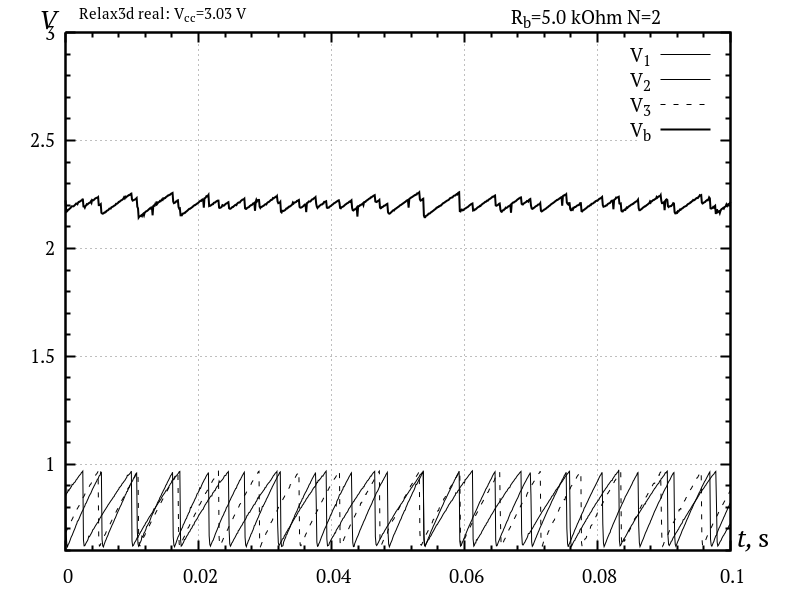
\includegraphics[width=0.6\textwidth]{p/relax3d_t_02.png} }
  \caption{Залежності $V_b(t)$, $V_i(t)$ для системи ``relax3d'' при $R_b=\SI{5.0}{\kilo\ohm}$ }
  \label{atu:f:relax3d_t_02}
\end{figure}


У цих умовах спектр
$ V_b (t) $ практично являє собою лінійну комбінацію спектрів (з
відповідними коефіцієнтами) окремих релаксаційних елементів,
тобто набір окремих частот~(рис.~\ref{atu:f:relax3d_f_02}, a). Аттрактор
системи при цьому має вигляд досить нетиповий для систем, які
не демонструють хаотичну динаміку (рис.~\ref{atu:f:relax3d_f_02}, b). Якщо
відношення частот релаксаційних елементів не є раціональним
числом, то аттрактор є кубом, щільно заповненим по кожній
координаті в діапазоні
$ [V \Tidx{off}; V \Tidx{on}] $.


\begin{figure}[htb!]
  \centerline{
    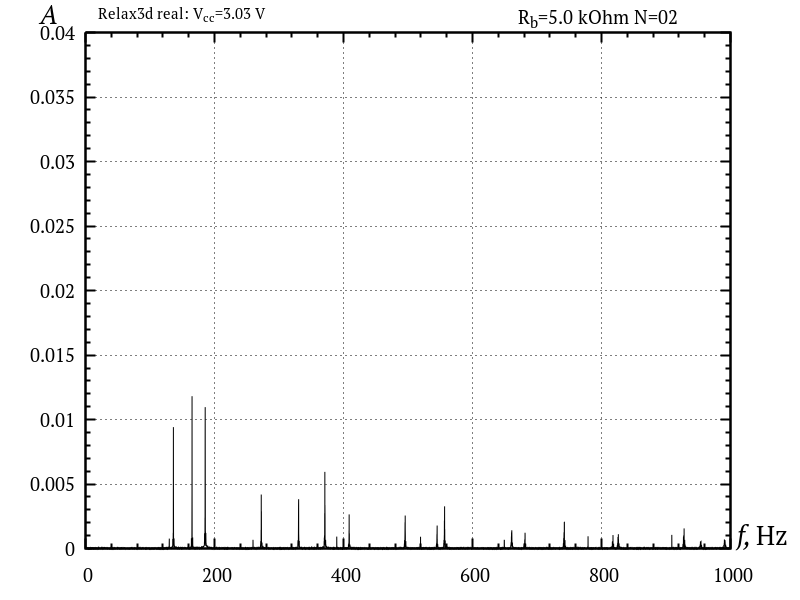
\includegraphics[width=0.48\textwidth]{p/relax3d_f_02.png}
    ~
    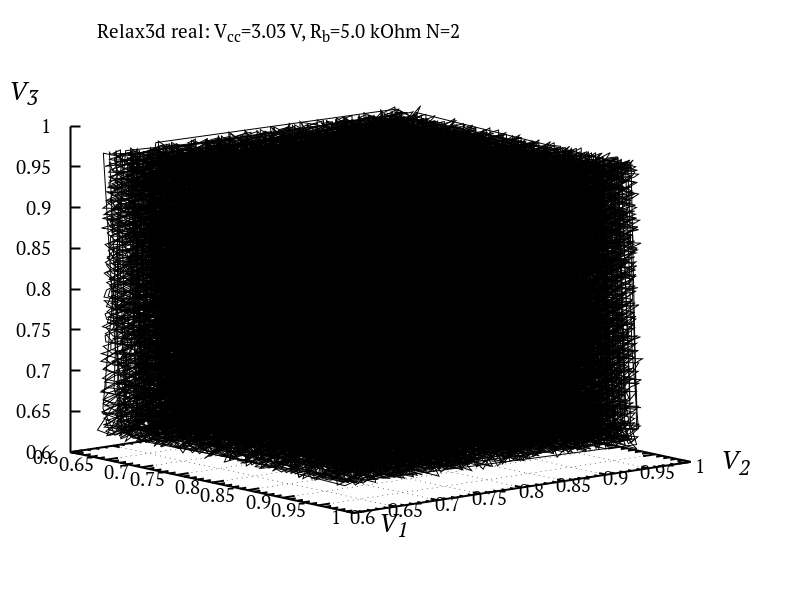
\includegraphics[width=0.48\textwidth]{p/relax3d_v1v2v3_02.png}
  }
\caption{Спектр $ V_b (t) $, і аттрактор для системи `` relax3d '' при $ R_b = \SI{5.0}{\kilo \ohm} $}
\label{atu:f:relax3d_f_02}
\end{figure}

При збільшенні
$R_b$ зв'язок між релаксаційним елементами стає сильнішим
(рис.~\ref{atu:f:relax3d_t_08}), і при цьому можлива ситуація, коли процес
заряду одного елемента настільки уповільнює момент перемикання
іншого, що це уповільнення впливає на всі елементи. Виникає стан
``перегонів'', коли перший переключився елемент істотно сповільнює
перемикання другого. Таким чином, виникає точка біфуркації,
коли малі зміни в початковому стані системи призводять до
істотних змін в подальшій динаміці. При сприятливих умовах
це може призводити до хаотичної поведінки.


\begin{figure}[htb!]
  \centerline{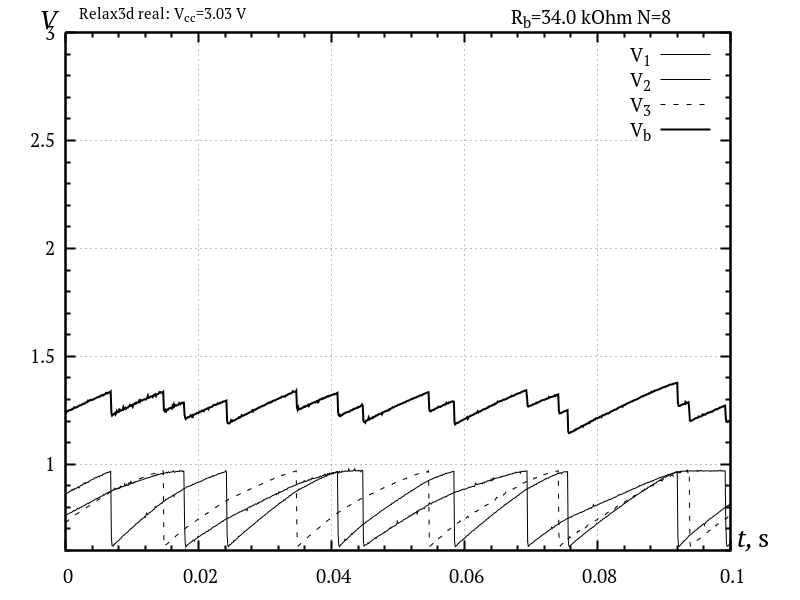
\includegraphics[width=0.6\textwidth]{p/relax3d_t_08.png} }
\caption{Залежності $ V_b (t) $, $ V_i (t) $ для системи ``relax3d'' при $ R_b = \SI{34.0}{\kilo\ohm} $}
\label{atu:f:relax3d_t_08}
\end{figure}

При цьому спектр системи має суцільні ділянки, підтверджуючи
хаотичність поведінки~(рис.~\ref{atu:f:relax3d_f_08}, a). Аттрактор ж
системи~(рис.~\ref{atu:f:relax3d_f_08}, b), навпаки, менш щільно заповнює
доступний простір.

\begin{figure}[htb!]
  \centerline{
    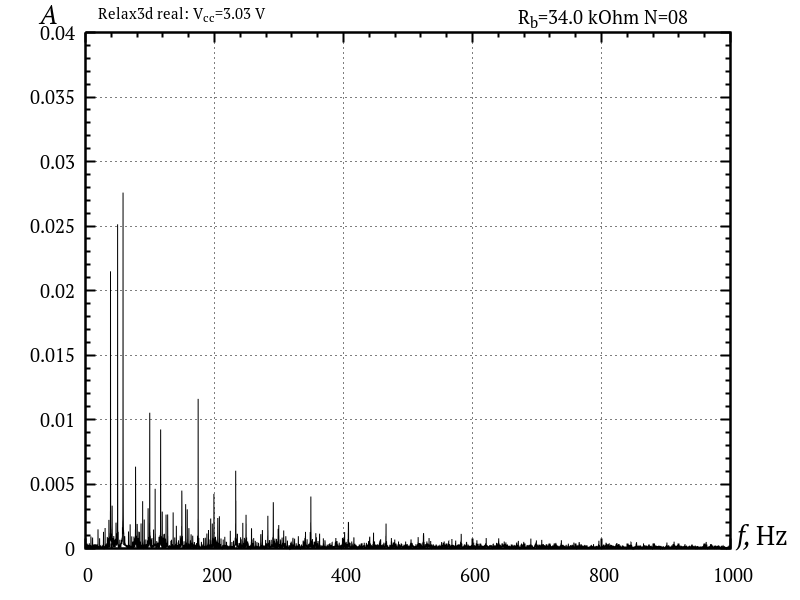
\includegraphics[width=0.48\textwidth]{p/relax3d_f_08.png}
    ~
    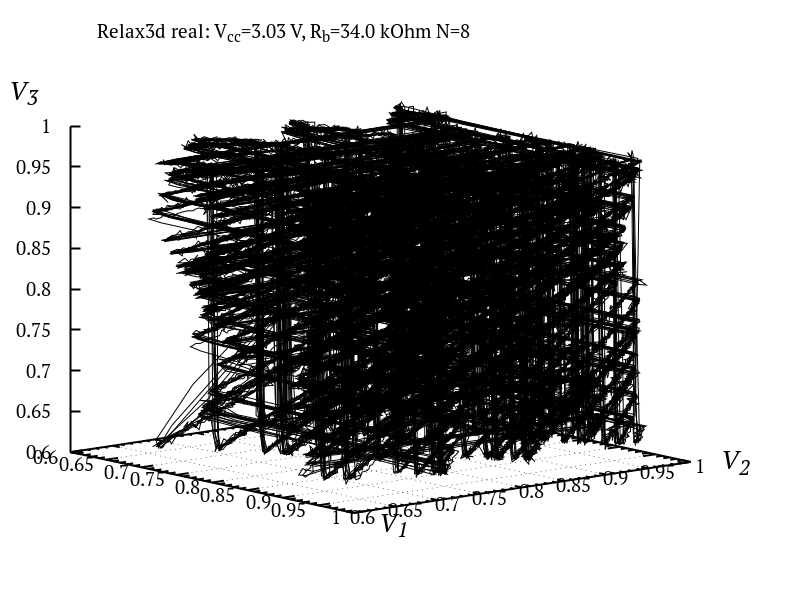
\includegraphics[width=0.48\textwidth]{p/relax3d_v1v2v3_08.png}
  }
\caption{Спектр $ V_b (t) $, і аттрактор для системи ``relax3d'' при $ R_b = \SI{34.0}{\kilo\ohm} $}
  \label{atu:f:relax3d_f_08}
\end{figure}

Однак, сильний зв'язок між релаксаційним елементами зовсім не
обов'язково призводить до хаотичної поведінки. При певних
умовах можлива самосинхронізація елементів генератора, тобто
створюються умови, еквівалентні раціональному ставленню частот
окремих генераторів. Наприклад, при подальшому збільшенні
$R_b$, знову виникає складно-періодичне
поведінка~(рис.~\ref{atu:f:relax3d_t_09}).

\begin{figure}[htb!]
  \centerline{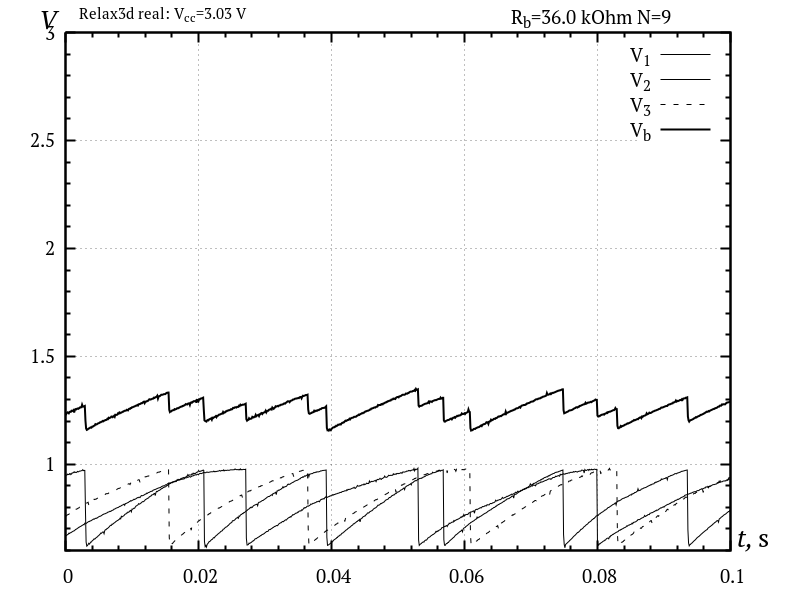
\includegraphics[width=0.6\textwidth]{p/relax3d_t_09.png} }
\caption{Залежності $ V_b (t) $, $ V_i (t) $ для системи ``relax3d'' при $ R_b = \SI{36.0}{\kilo\ohm} $}
\label{atu:f:relax3d_t_09}
\end{figure}

Спектр системи стає лінійчатим (рис.~\ref{atu:f:relax3d_f_09}, a), при
цьому часто спостерігається рівні відстані між піками
частот. Аттрактор стає більш виродженим~(рис.~\ref{atu:f:relax3d_f_09}, b).

\begin{figure}[htb!]
  \centerline{
    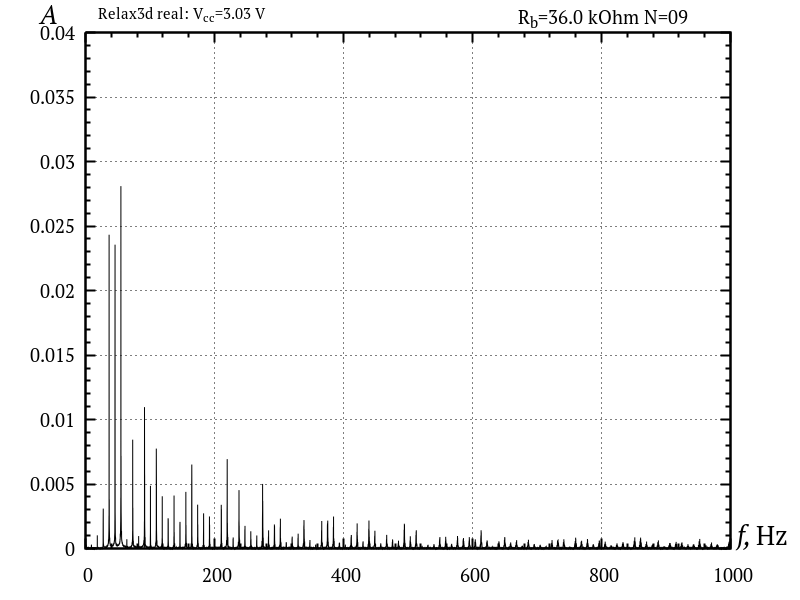
\includegraphics[width=0.48\textwidth]{p/relax3d_f_09.png}
    ~
    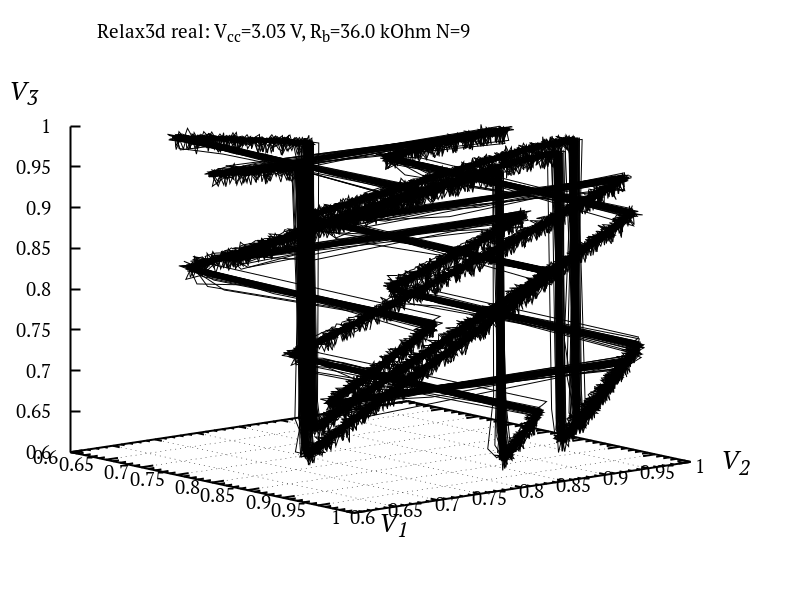
\includegraphics[width=0.48\textwidth]{p/relax3d_v1v2v3_09.png}
  }
  \caption{Спектр $V_b(t)$, и аттрактор для системи ``relax3d'' при $R_b=\SI{36.0}{\kilo\ohm}$ }
  \label{atu:f:relax3d_f_09}
\end{figure}

З подальшим зростанням значення параметра
$R_b$, складно-періодичний і хаотичний режими чергуються. Зрештою,
виникає режим, коли один з релаксаційних елементів припиняє
генерацію~(рис.~\ref{atu:f:relax3d_t_22}). Цей момент настає значно раніше,
ніж передбачає модель. Це пов'язано з тим, що застосований в даній
схемі елемент, що перемикає, при малих токах починає працювати
як стабілізатор напруги.

\begin{figure}[htb!]
  \centerline{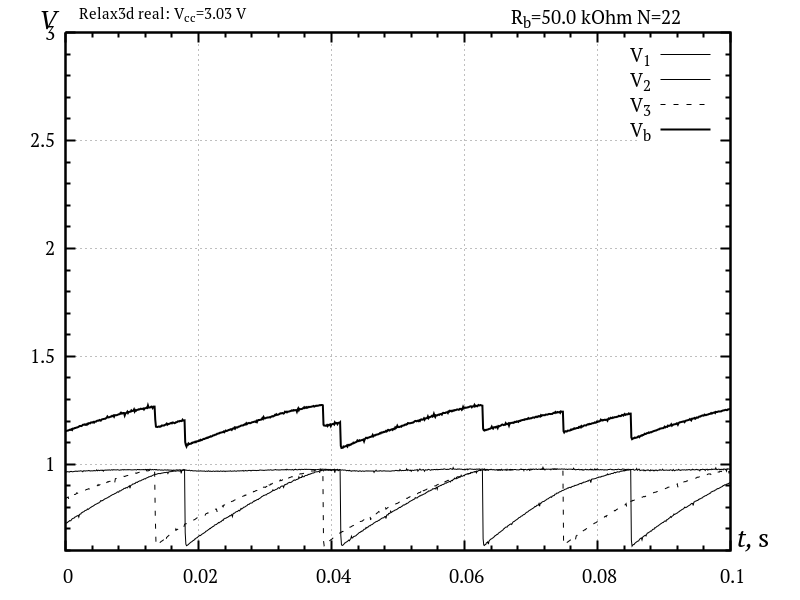
\includegraphics[width=0.6\textwidth]{p/relax3d_t_22.png} }
\caption{Залежності $ V_b (t) $, $ V_i (t) $ для системи ``relax3d'' при $ R_b = \SI{50.0}{\kilo \ohm} $}
\label{atu:f:relax3d_t_22}
\end{figure}

Два робочих релаксаційних елемента забезпечують досить
бідний лінійчатий спектр~(рис.~\ref{atu:f:relax3d_f_22}, a). Аттрактор при
цьому втрачає один з вимірів~(рис.~\ref{atu:f:relax3d_f_22}, b), відповідний
виключеному зі генерації елементу.

\begin{figure}[htb!]
  \centerline{
    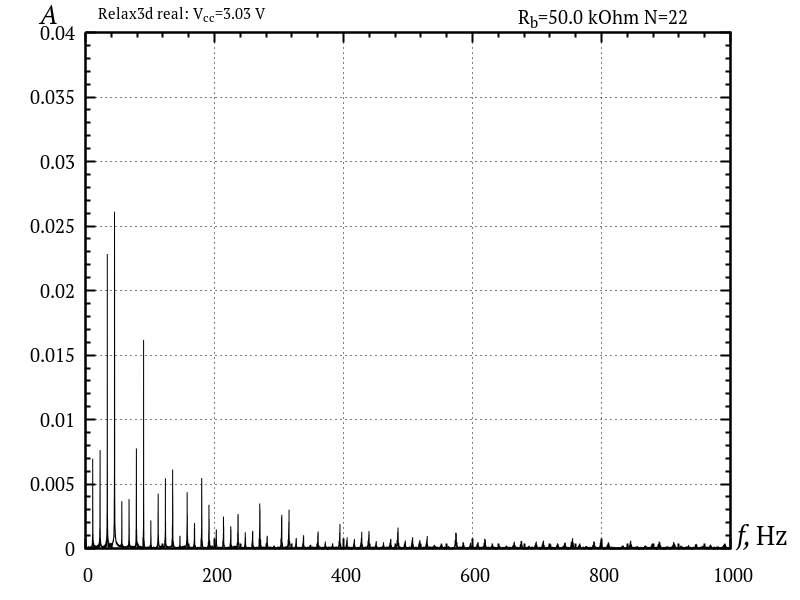
\includegraphics[width=0.48\textwidth]{p/relax3d_f_22.png}
    ~
    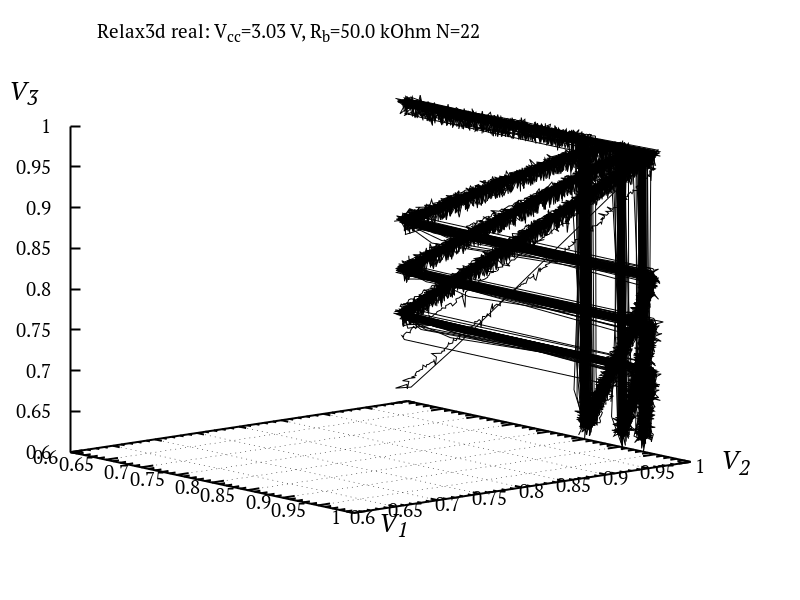
\includegraphics[width=0.48\textwidth]{p/relax3d_v1v2v3_22.png}
  }
\caption{Спектр $ V_b (t) $, і аттрактор для системи ``relax3d'' при $ R_b = \SI{50.0}{\kilo \ohm} $}
\label{atu:f:relax3d_f_22}
\end{figure}

Таким чином встановлено, що система ``relax3d'', електрична схема
якої приведена на рис.~\ref{atu:f:relax3d_schem}, в інтервалі значень
параметра
$ R_b \in [1; 50] \; \SI{}{ \kilo \ohm} $ демонструє як складно-періодичну,
так і хаотичну поведінку, причому режими мають тенденцію до
чергування.

\section{Система з трьох пов'язаних релаксаційних генераторів на основі тригерів Шмідта}
\label{atu:sec:relax3ds}

Схемотехнічна реалізація системи пов'язаних релаксаційних
генераторів, розглянута в розділі \ref{atu:sec:relax3d}, незважаючи на
ряд переваг, має певні недоліки. В першу чергу, слід відзначити
той факт, що при відносно високих значеннях величини
$ R_b $, якраз при яких зв'язок між окремими генераторами стає
істотним, релаксаційний елемент перемикається з коливального
режиму в режим стабілізації напруги, що не відповідає
призначенню даної схеми. Більш того, в цих умовах залежність
струму від напруги близька до експоненційної, що ускладнює
створення адекватної моделі. При цьому малі зміни параметрів,
наприклад, викликані температурною нестабільністю, призводять
до значних змін струму, що також негативно впливає
на адекватність. Ще один недолік полягає в тому, що існуючими
елементами можна змінювати напругу спрацьовування в досить
вузькому діапазоні, що ускладнює проведення як експериментів,
так і моделювання в широкому діапазоні параметрів. У свою чергу,
це ставить додаткові питання про межі застосування моделі, на
які складно відповісти, спираючись на результати експерименту.

Таким чином, виникає задача синтезу схеми системи пов'язаних
релаксаційних генераторів, яка б в мінімальному ступені була
б схильною до вищезгаданих недоліків.

Один з досить очевидних способів полягає в поділі
елемента, що перемикає, на вимірювальну і перемикаючу частини. Як
частину, що перемикає, можна продовжити використовувати біполярний
транзистор. Використання MOSFET транзистора може дозволити значно
зменшити опір ланцюга розряду, однак, з огляду на вимогу до
низьку напругу живлення, забезпечити повне відкриття такого
транзистора без застосування спеціальних драйверів досить
складно, а спеціальні драйвери вимагають окремого живлення,
що вимагає певних запобіжних заходів при підключенні АЦП, і,
в свою чергу, можуть вносити додаткові спотворення сигналу.

В якості вимірювального елемента можна використовувати
відповідну за умовами бістабільності схему, чутливу до напруги,
наприклад тригер Шмідта. Якщо існує необхідність управляти
значеннями величин
$ V \Tidx{on} $,
$ V \Tidx{off} $, то тригер слід реалізовувати, використовуючи
операційні підсилювачі~\cite{horowitz}. При фіксованих значеннях
цих параметрів, можна використовувати тригери Шмідта в
інтегральному виконанні, вибрав відповідну серію. З
урахуванням вищезазначених вимог, були обрані мікросхеми
серії 74HC14N, що представляють собою 6 елементів ``NOT'' з тригером
Шмідта на вході. Комбінуючи їх по два, отримаємо три необхідні
вимірювальні елемента. Отримана схема представлена на
рис.~\ref{atu:f:relax3ds_schem}.


\begin{figure}[htb!]
  \centerline{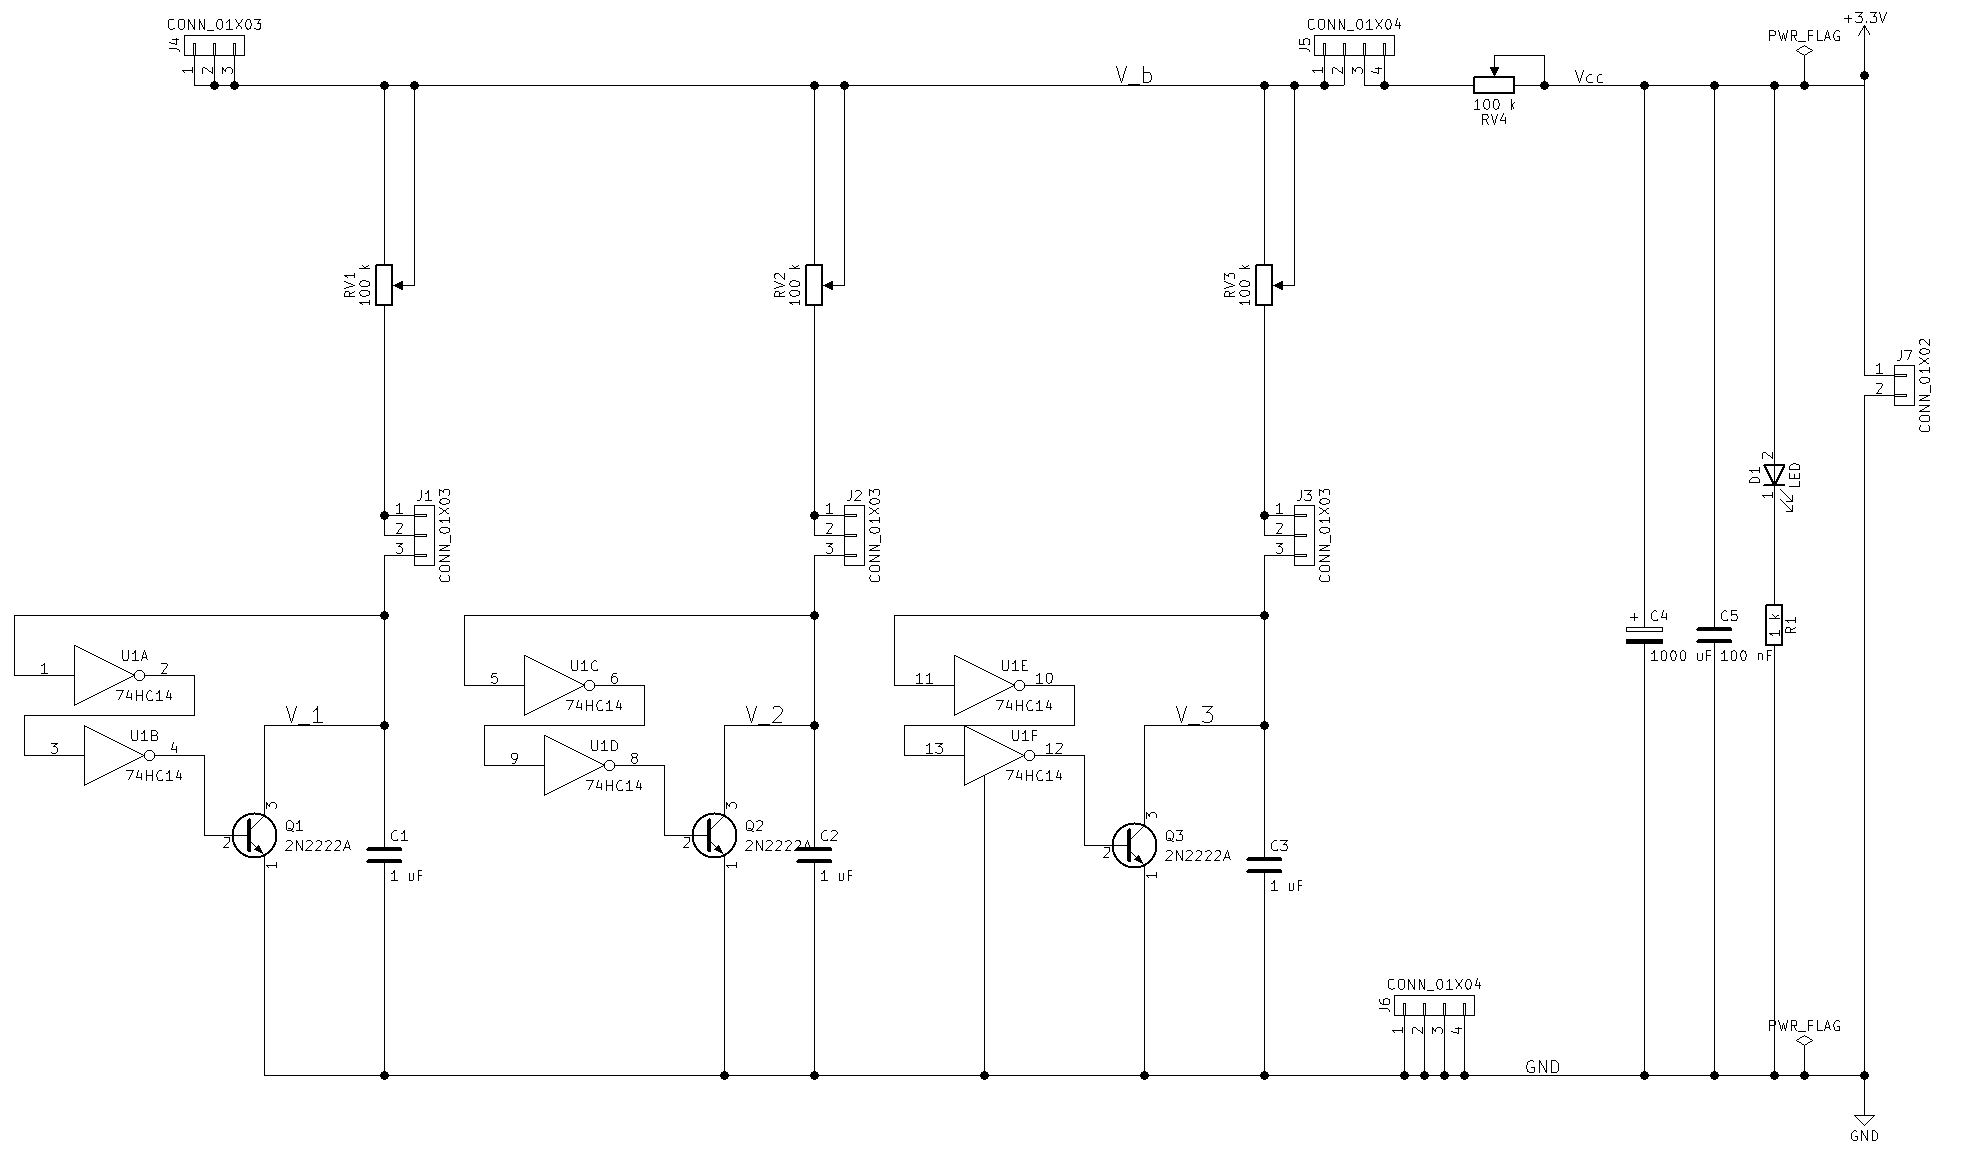
\includegraphics[width=0.9\textwidth]{p/relax3ds_schem.png} }
\caption{Електрична схема \RelaxShIi}
\label{atu:f:relax3ds_schem}
\end{figure}

Принципово ця схема не відрізняється від зображеної
на рис.~\ref{atu:f:relax3d_schem}. Всі допоміжні елементи виконують
аналогічну роль. При цьому існують і певні відмінності. Напруги
спрацьовування  елемента, що перемикає, у даної схеми
відрізняються, і визначаються параметрами тригера. Згідно з
документацією, для зазначеної мікросхеми при
$ V \Tidx{cc} = \SI{3}{\volt} $ допустимі діапазони визначаються так:$ V \Tidx{off}
\in [0.51; 1.35]~\SI{}{\volt} $,
$ V \Tidx{on} \in [1.08; 2.16]~\SI{}{\volt} $. Діапазони істотно відрізняються
від таких для попередньої схеми. Більш того, розкид допустимих
параметрів дуже широкий, і, теоретично, можливо ситуація, коли
деякі з релаксаційних елементів не будуть працювати. Проте,
при реальних вимірах для одного конкретного екземпляра розкид
виявився не такий великий:
$ V \Tidx{off, 1} = \SI{1.10}{\volt} $,
$ V \Tidx{off, 2} = \SI{1.05}{\volt} $,
$ V \Tidx{off, 3} = \SI{1.02}{\volt} $,
$ V \Tidx{on, 1} = \SI{1.87}{\volt} $ ,
$ V \Tidx{on, 2} = \SI{1.83}{\volt} $,
$ V \Tidx{on, 3} = \SI{1.81}{\volt} $. Відмінності, незважаючи на те, що вони
помітно менше, ніж допустимі по офіційній документації, проте
істотно більше, ніж в попередній схемі, що вимагає обов'язкового
врахування в моделі.

Дану схемотехнічну реалізацію в подальшому будемо позначати як ``relax3ds''.

Зовнішній вигляд зібраної схеми на макетної платі
представлено на рис.~\ref{atu:f:relax3ds_board}.

\begin{figure}[htb!]
  \centerline{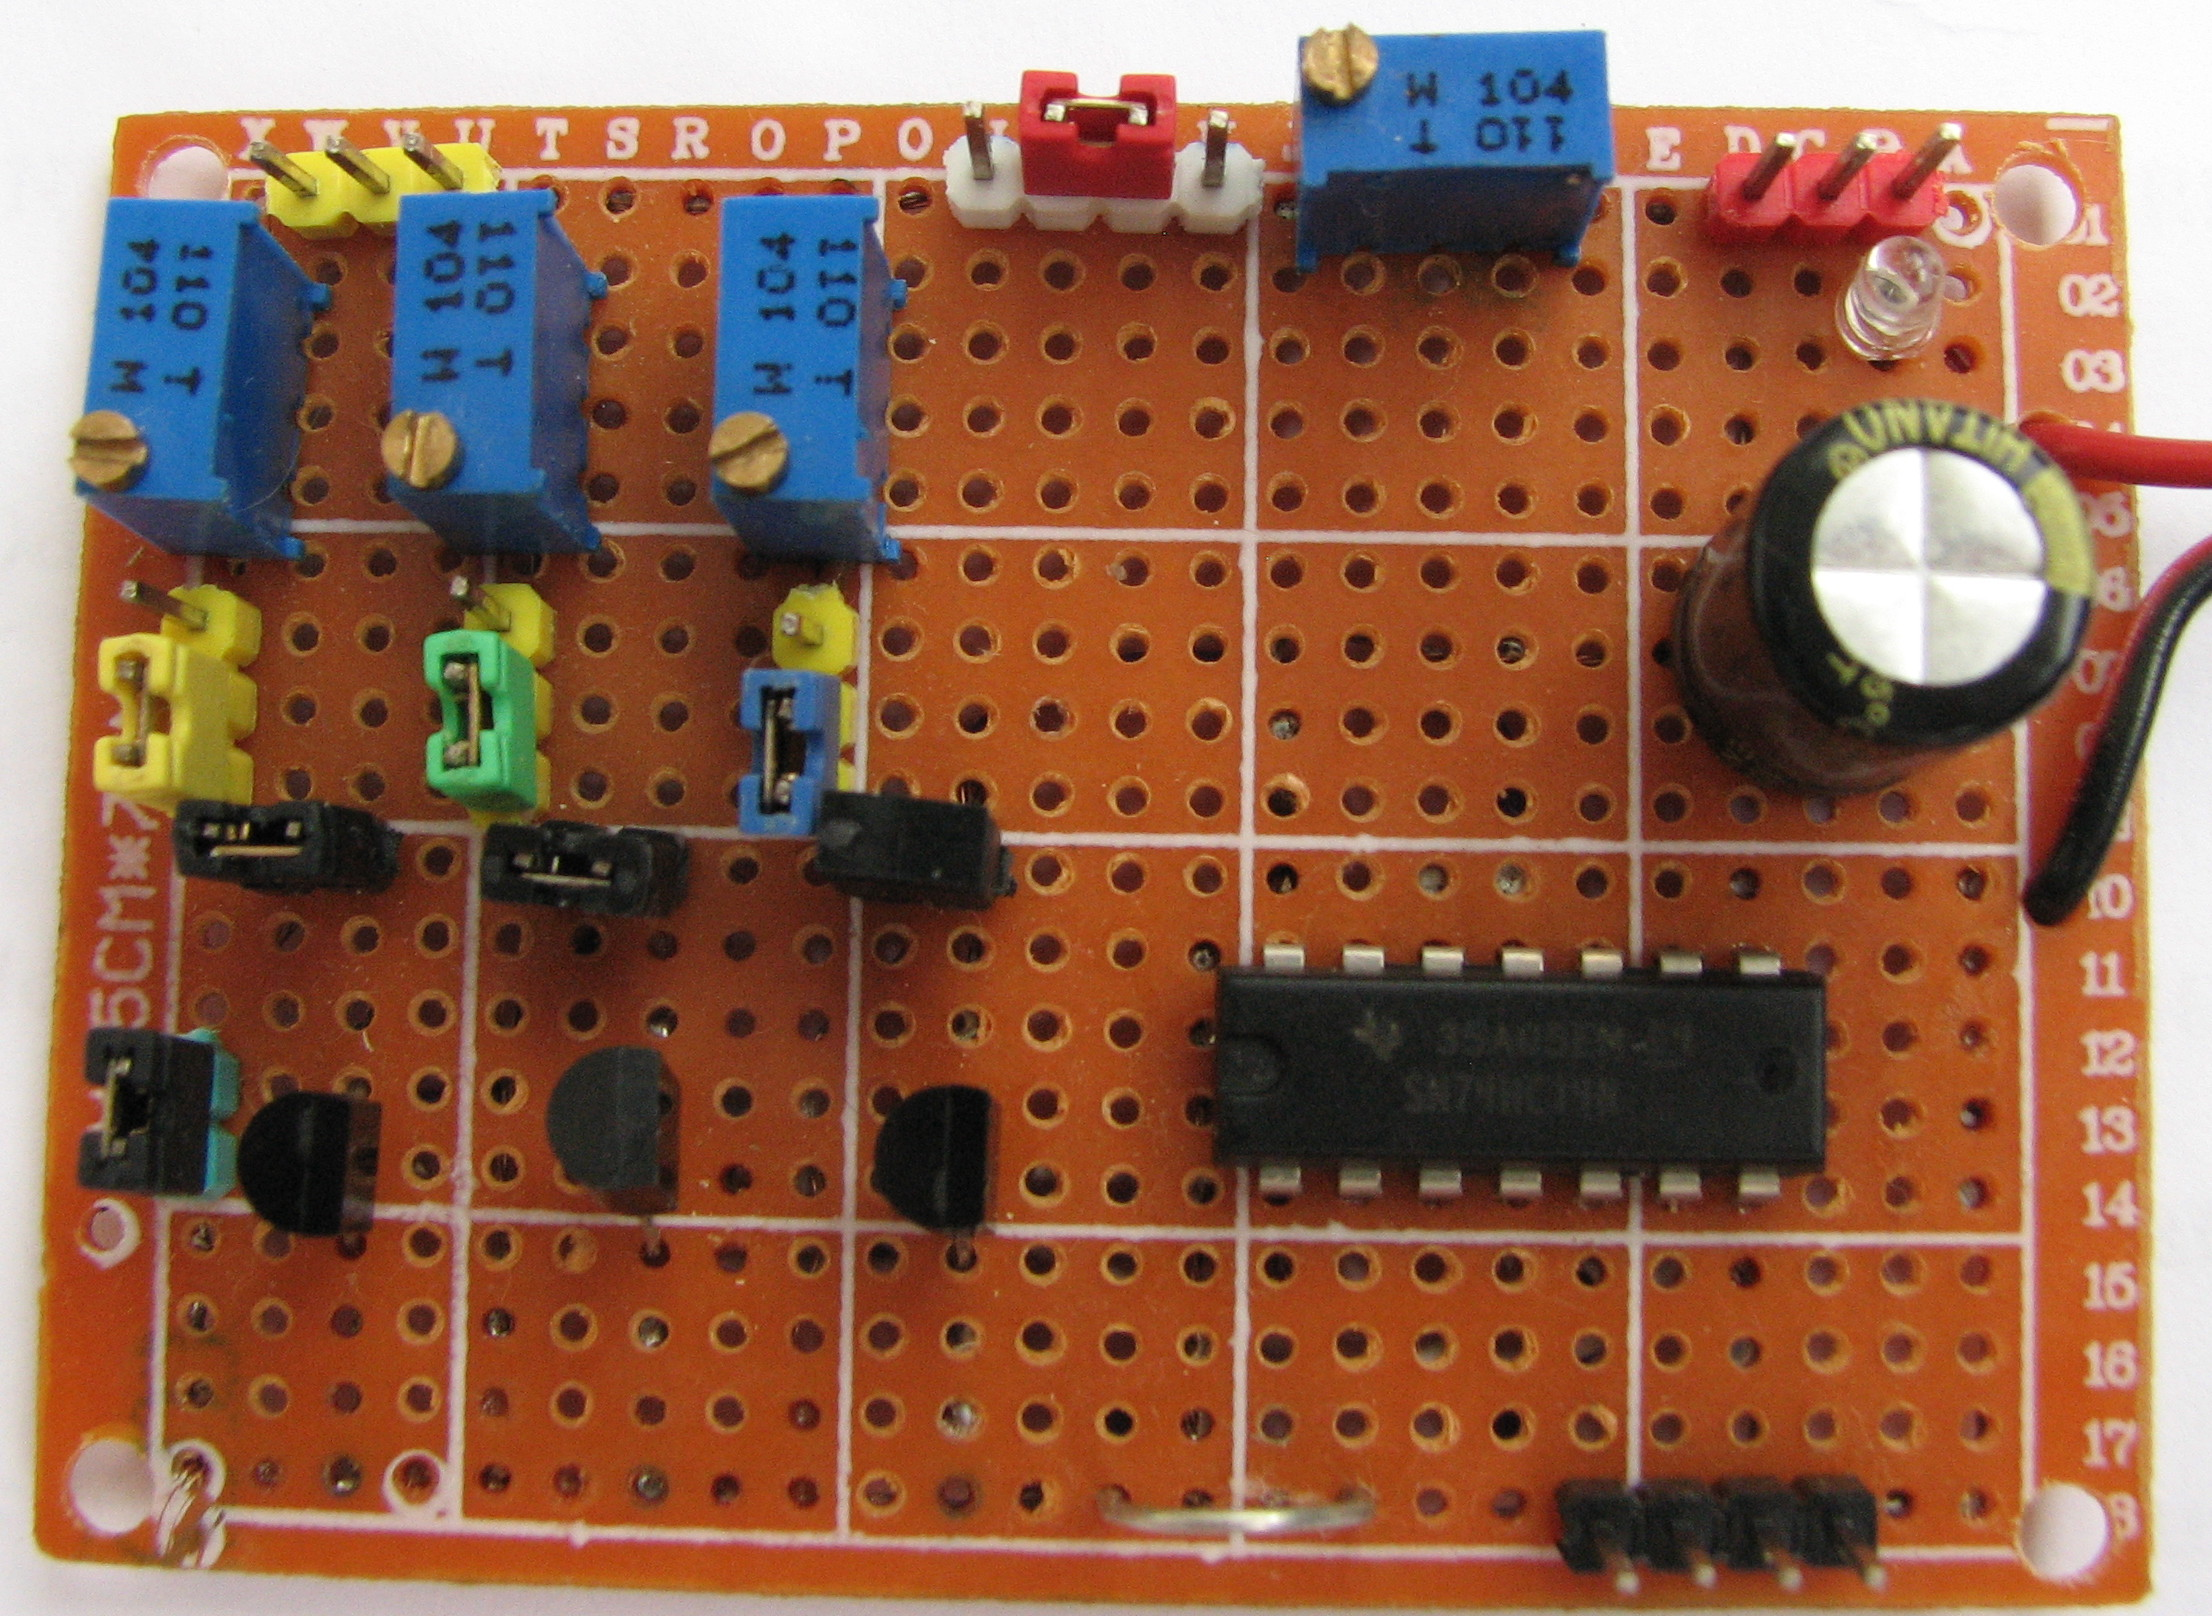
\includegraphics[width=0.6\textwidth]{p/relax3ds_board.jpg} }
\caption{Схема (рис.~\ref{atu:f:relax3ds_schem}), зібрана на макетної платі}
\label{atu:f:relax3ds_board}
\end{figure}

Аналогічно попередній схемі, розглянемо її динаміку при зміні
$ R_b $, виділяючи аналогічні режими.

При малих значеннях
$ R_b $ абсолютно аналогічно спостерігаються практично незалежні
коливання~(рис.~\ref{atu:f:relax3ds_t_05151}). Однак, через підвищення напруги
перемикання, коливання величини
$ V \Tidx{b} $ виражені сильніше.

\begin{figure}[htb!]
  \centerline{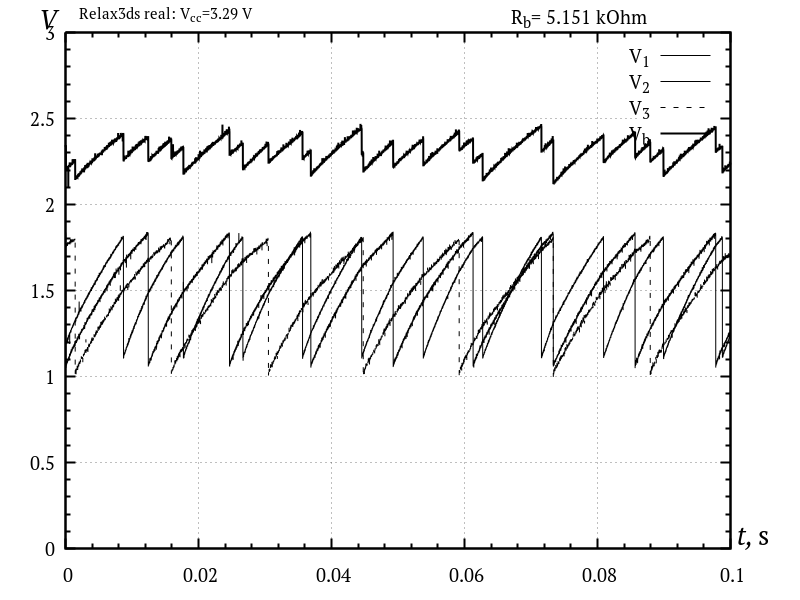
\includegraphics[width=0.6\textwidth]{p/relax3ds_t_005151.png} }
\caption{Залежності $ V_b (t) $, $ V_i (t) $ для системи ``relax3ds'' при $ R_b = \SI{5.15}{\kilo \ohm} $}
  \label{atu:f:relax3ds_t_05151}
\end{figure}


Через більш сильний зв'язок між елементами, спостерігається
розширення спектральних ліній~(рис.~\ref{atu:f:relax3ds_f_05151}). Аттрактор
--- прямокутний паралелепіпед, досить щільно заповнений по кожній
координаті в діапазоні
$ [V \Tidx{off, i}; V \Tidx{on, i}] $.


\begin{figure}[htb!]
  \centerline{
    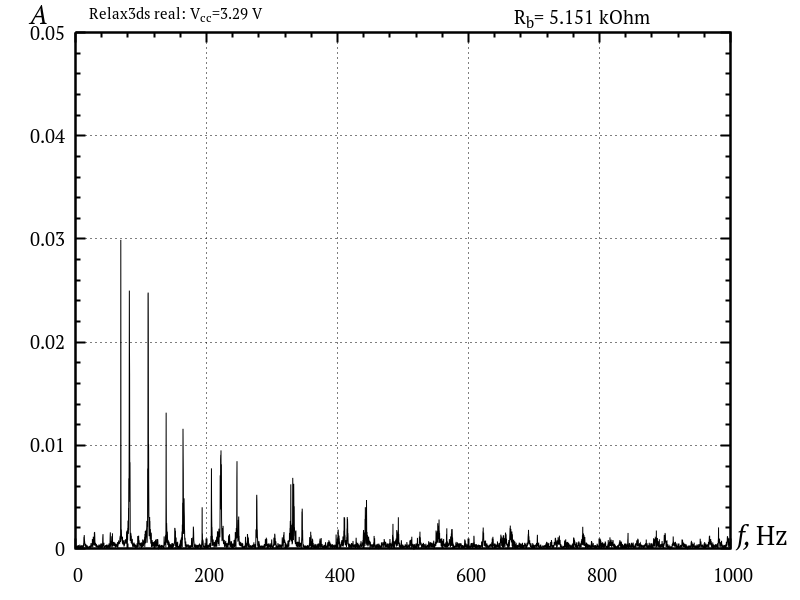
\includegraphics[width=0.48\textwidth]{p/relax3ds_f_005151.png}
    ~
    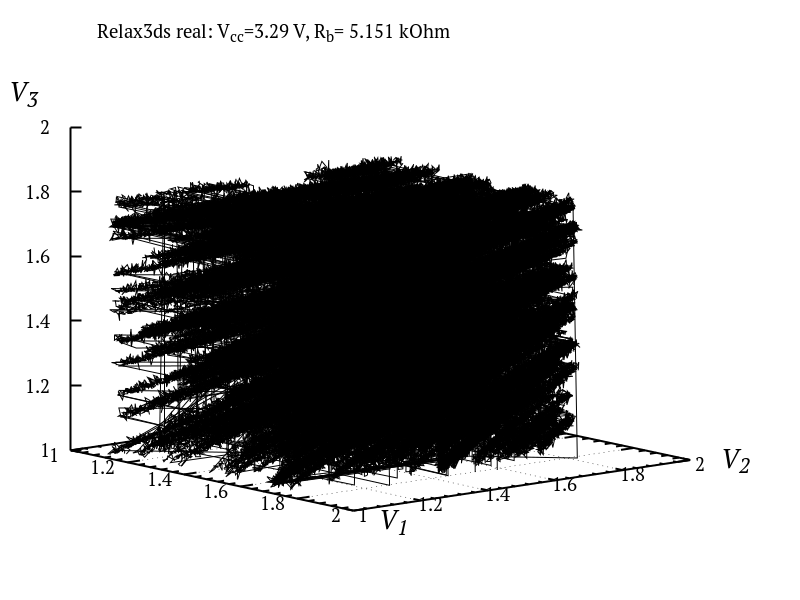
\includegraphics[width=0.48\textwidth]{p/relax3ds_v1v2v3_005151.png}
  }
\caption{Спектр $ V_b (t) $, і аттрактор для системи `` relax3ds '' при $ R_b = \SI{5.15}{\kilo \ohm} $}
\label{atu:f:relax3ds_f_05151}
\end{figure}

Посилення зв'язку призводить до вираженої хаотичного поведінки
(рис.~\ref{atu:f:relax3ds_t_13246}).

\begin{figure}[htb!]
  \centerline{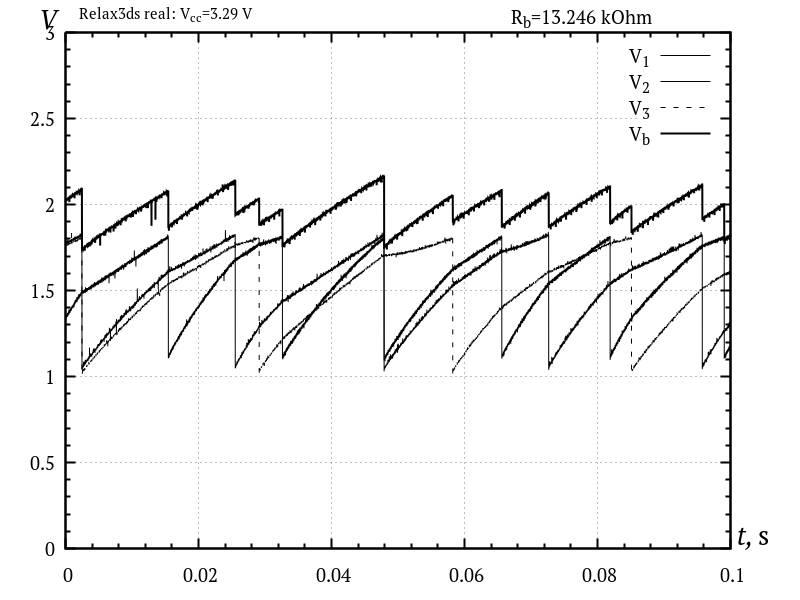
\includegraphics[width=0.6\textwidth]{p/relax3ds_t_013246.png} }
  \caption{Залежності $V_b(t)$, $V_i(t)$ для системи ``relax3ds'' при $R_b = \SI{13.25}{\kilo\ohm} $}
  \label{atu:f:relax3ds_t_13246}
\end{figure}

Суцільні ділянки спектра~(рис.~\ref{atu:f:relax3ds_f_13246}, a)
є хорошим індикатором хаосу. Аттрактор виглядає
аналогічно~(рис.~\ref{atu:f:relax3ds_f_13246}, b).

\begin{figure}[htb!]
  \centerline{
    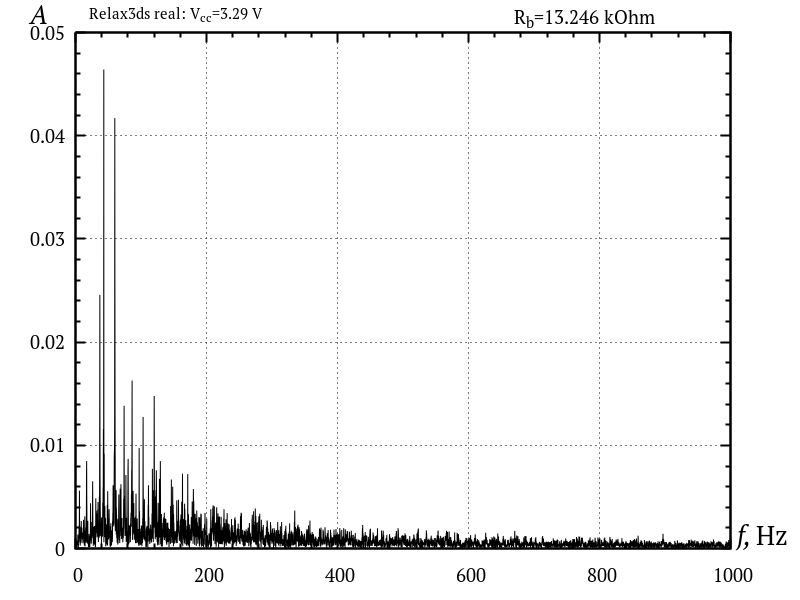
\includegraphics[width=0.48\textwidth]{p/relax3ds_f_013246.png}
    ~
    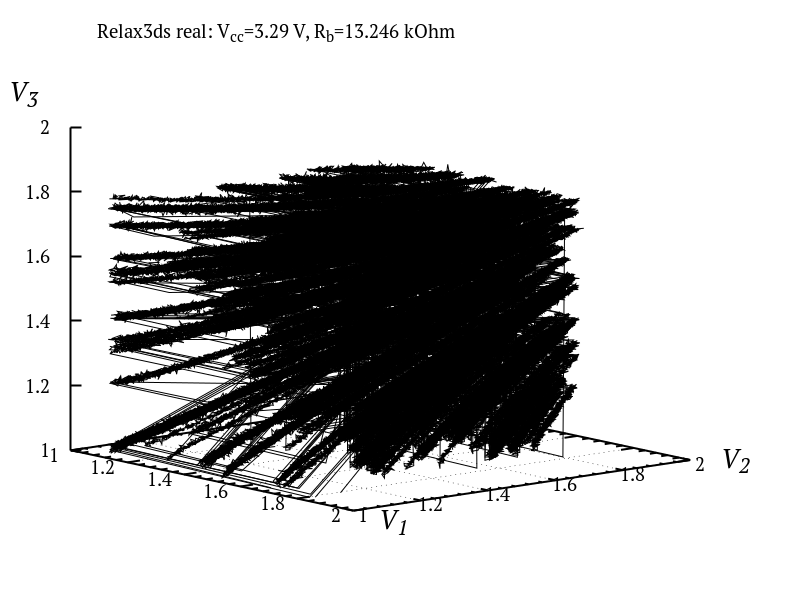
\includegraphics[width=0.48\textwidth]{p/relax3ds_v1v2v3_013246.png}
  }
  \caption{Спектр $V_b(t)$, і аттрактор для системи ``relax3ds'' при $R_b=\SI{5.15}{\kilo \ohm} $}
  \label{atu:f:relax3ds_f_13246}
\end{figure}

Певні значення
$R_b$ переводять систему в складно-періодичний режим (рис.~\ref{atu:f:relax3ds_t_14718}).

\begin{figure}[htb!]
  \centerline{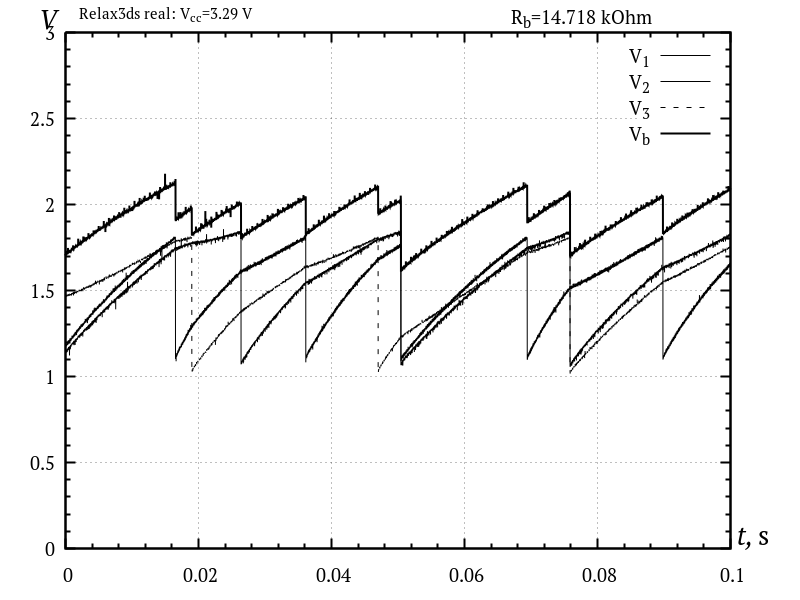
\includegraphics[width=0.6\textwidth]{p/relax3ds_t_014718.png} }
  \caption{Залежності $V_b(t)$, $V_i(t)$ для системи ``relax3ds'' при $R_b=\SI{14.72}{\kilo\ohm} $}
  \label{atu:f:relax3ds_t_14718}
\end{figure}

Спектр~(рис.~\ref{atu:f:relax3ds_f_14718}, a) підтверджує відсутність хаосу,
незважаючи на тонку лінійчату структуру. Аттрактор принципово
не змінюється~(рис.~\ref{atu:f:relax3ds_f_14718}, b), але має менш щільне
заповнення.

\begin{figure}[htb!]
  \centerline{
    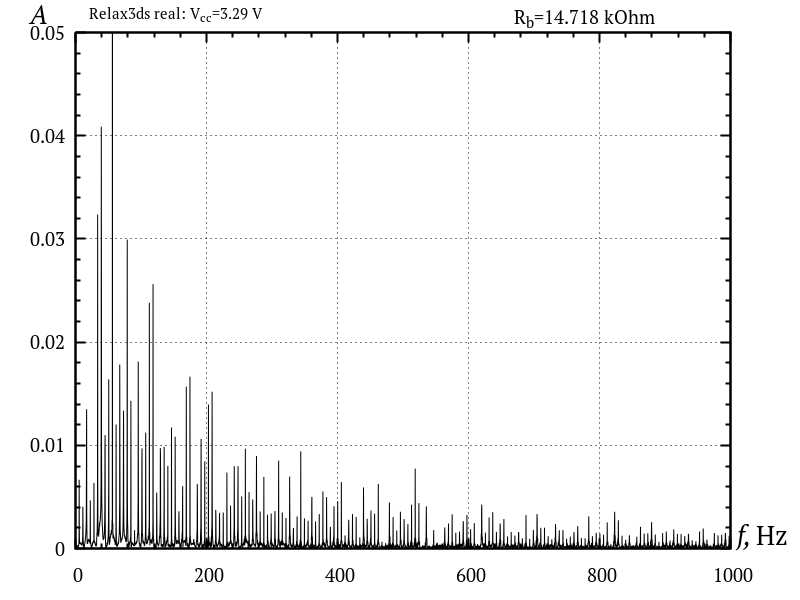
\includegraphics[width=0.48\textwidth]{p/relax3ds_f_014718.png}
    ~
    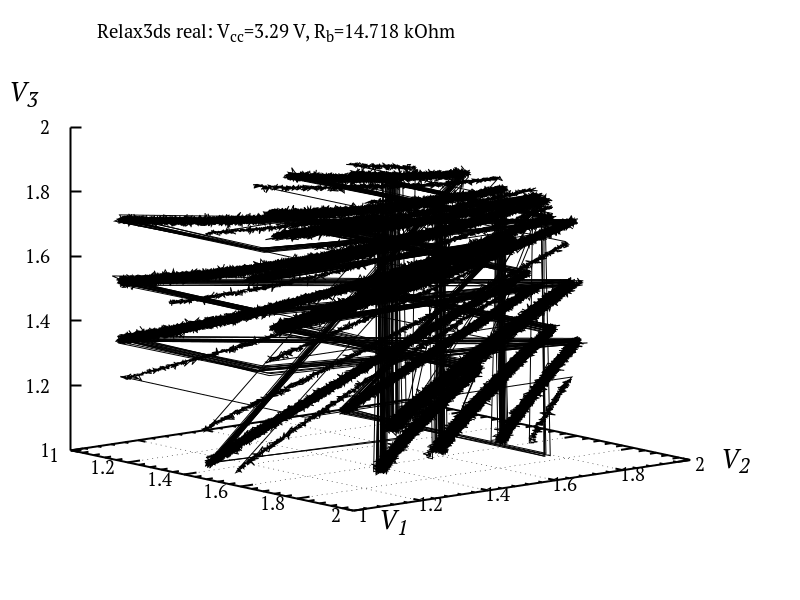
\includegraphics[width=0.48\textwidth]{p/relax3ds_v1v2v3_014718.png}
  }
  \caption{Спектр $V_b(t)$, і аттрактор для системи ``relax3ds'' при $R_b=\SI{14.72}{\kilo \ohm} $}
  \label{atu:f:relax3ds_f_14718}
\end{figure}

Високі значення
$ R_b $, на відміну від попередньої системи, не приводять до швидкого
виключення одного з релаксаційних елементів, при цьому може
спостерігатися як складно-періодичне, так і хаотична поведінка
(рис.~\ref{atu:f:relax3ds_t_36060}).

\begin{figure}[htb!]
  \centerline{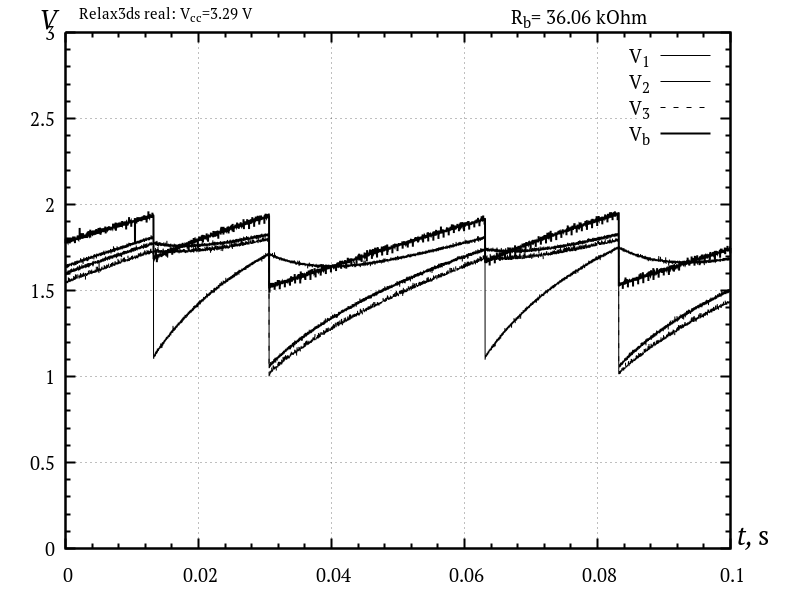
\includegraphics[width=0.6\textwidth]{p/relax3ds_t_036060.png} }
  \caption{Залежності $V_b(t)$, $V_i(t)$ для системи ``relax3ds'' при $R_b = \SI{36.06}{\kilo\ohm} $}
  \label{atu:f:relax3ds_t_36060}
\end{figure}

Спектри можуть бути як суцільними~(рис.~\ref{atu:f:relax3ds_f_36060},
a) так і лінійчатими. Аттрактори мають більш просту
структуру~(рис.~\ref{atu:f:relax3ds_f_36060}, b), при цьому реалізовуючи як
і прості еквіваленти фігур Ліссажу, так і фігури з щільним
заповненням.

\begin{figure}[htb!]
  \centerline{
    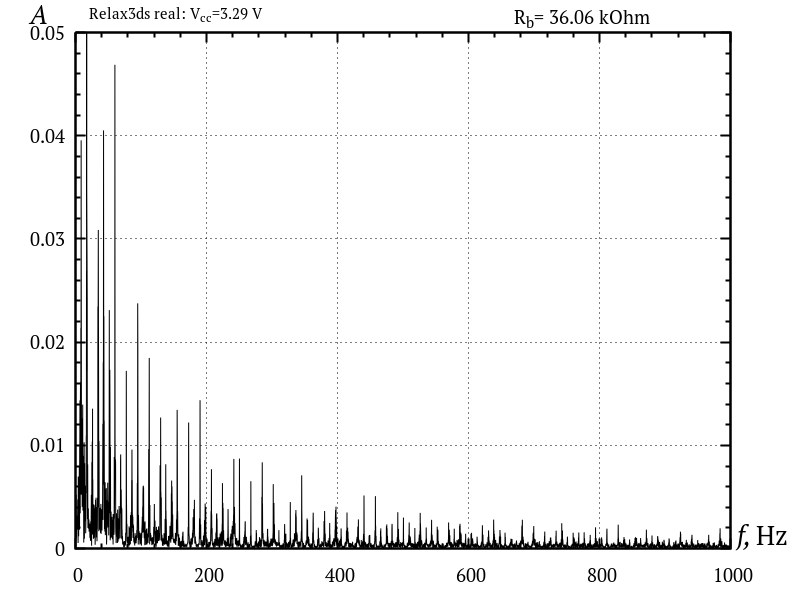
\includegraphics[width=0.48\textwidth]{p/relax3ds_f_036060.png}
    ~
    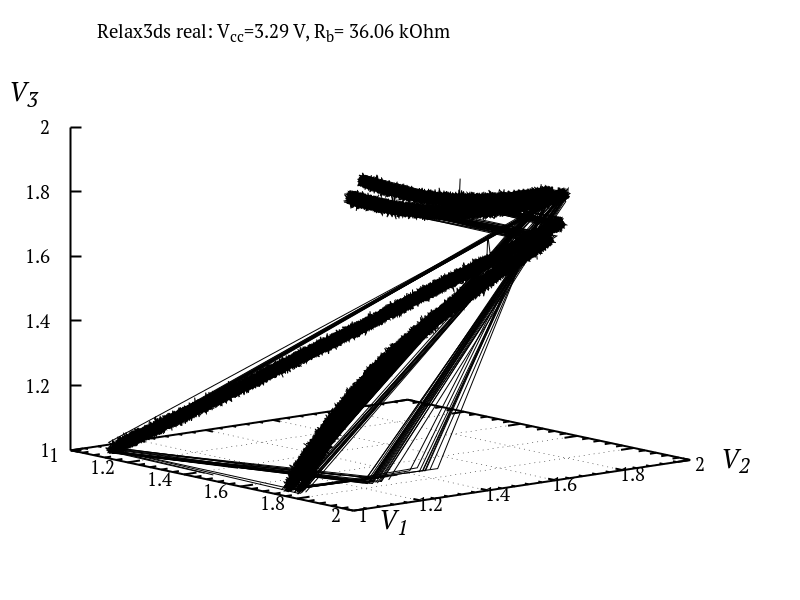
\includegraphics[width=0.48\textwidth]{p/relax3ds_v1v2v3_036060.png}
  }
  \caption{Спектр $V_b(t)$, і аттрактор для системи ``relax3ds'' при $R_b=\SI{36.06}{\kilo \ohm} $}
  \label{atu:f:relax3ds_f_36060}
\end{figure}

В цілому обидві схеми, незважаючи на відмінності, мають подібні
принципи поведінки в досить широкому діапазоні значень
параметра
$R_b$. Істотна різниця проявляється при високих значеннях
$R_b$, при цьому, очевидно, потрібно або уточнення моделі, або ж
невикористання даних режимів, які в цьому контексті не уявляють
особливого інтересу.


Порівняння динаміки систем ``relax3d'' і ``relax3ds'' дозволяє зробити
спостереження, що за інших рівних перша з них демонструє менший
рівень зв'язку між релаксаційним елементами. Тобто для отримання
аналогічного поведінки для другої системи слід задавати менші
значення
$ R_b $. Це пов'язано великим значенням безрозмірною величини
$ v $ для другої системи, через відносно великих значень
$ V \Tidx{off} $,
$ V \Tidx{on} $.


\section{Моделі систем з трьох пов'язаних релаксаційних генераторів}

З урахуванням вищевикладеного, модель системи пов'язаних
релаксаційних генераторів можна представити в наступному
вигляді:
%
\begin{equation}
  \begin{cases}
    V_b = V_{cc} - R_b ( I_1 + I_2 + I_3 ), \\
      C_1 \dot{V}_1 = \frac{V_b-V_1}{R_{v1}} - \frac{V_1}{R_1} \mathrm{On}_1() - I_{1,\mathrm{leak}}(V_1), \\
      C_2 \dot{V}_2 = \frac{V_b-V_2}{R_{v2}} - \frac{V_2}{R_2} \mathrm{On}_2() - I_{2,\mathrm{leak}}(V_2), \\
      C_3 \dot{V}_3 = \frac{V_b-V_3}{R_{v3}} - \frac{V_3}{R_3} \mathrm{On}_3() - I_{3,\mathrm{leak}}(V_3), \\
      I_i = \frac{V_b-V_i}{R_{vi}}.
  \end{cases}.
    \label{atu:eq:relax3}
\end{equation}
%
де: \\
$ R_b $ --- опір в ланцюзі живлення (ідентифікований параметр), \\
$ C_i $ --- ємності кожного з релаксаційних генераторів, \\
$ R_{vi} $ --- опору зарядки релаксаційних генераторів, \\
$ R_{ i} $ --- опору зарядки релаксаційних генераторів, \\
$ I_{i, \mathrm{leak}} $ --- струми витоку.


Функції
$ \mathrm{On}_i() $ визначають моменти спрацьовування  елементів, що перемикають,
і з огляду на їх релейно-гістерезисний вид
задаються алгоритмічно. Визначальними параметрами при цьому є
$ V_{\mathrm{on}, i} $,
$ V_{\mathrm{off}, i} $.

У загальному випадку струми витоку
$ I_{i, \mathrm{leak}} $ описуються нелінійними функціями. У найпростіших
випадках витік можна моделювати через омічний опір:
%
\begin{equation}
  \begin{cases}
    V_b = V_{cc} - R_b ( I_1 + I_2 + I_3 ), \\
      C_1 \dot{V}_1 = \frac{V_b-V_1}{R_{v1}} - \frac{V_1}{R_1} \mathrm{On}_1() - \frac{V_1}{R_1+R_{1,\mathrm{leak}}}, \\
      C_2 \dot{V}_2 = \frac{V_b-V_2}{R_{v2}} - \frac{V_2}{R_2} \mathrm{On}_2() - \frac{V_2}{R_2+R_{2,\mathrm{leak}}}, \\
      C_3 \dot{V}_3 = \frac{V_b-V_3}{R_{v3}} - \frac{V_3}{R_3} \mathrm{On}_3() - \frac{V_3}{R_3+R_{3,\mathrm{leak}}}, \\
      I_i = \frac{V_b-V_i}{R_{vi}}.
  \end{cases}.
    \label{atu:eq:relax3_linleak}
\end{equation}
%
де
$ R_{i, \mathrm{leak}} $ --- опору витоку. При цьому досить часто виконується
співвідношення
$ R_{i} \ll R_{i, \mathrm{leak}} $, і величинами
$ R_{i} $ можна знехтувати. При виконанні умов
$ V_b \gg V_i $ струмами витоку можна знехтувати зовсім, однак для
хаотичних режимів виконання цієї умови нехарактерно, так як
вона передбачає слабий зв'язок між генераторами. Конкретний
вид витоку слід вибирати, виходячи з поведінки системи за умови
$ V_b \approx V_i $.

Перед тим, як приступити до моделювання системи пов'язаних
генераторів, необхідно переконається, що результати
чисельного моделювання показують адекватні результати в
тому випадку, коли можливо порівняти результати не тільки з
експериментом, але і з теоретичними розрахунками, тобто для
одного генератора. Для проведення цієї перевірки в системі
``relax3d'' були відключені другий і третій генератори. При цьому,
немає необхідності відстежувати сигнал
$ V_b (t) $, і в цьому експерименті під величиною
$ R_1 $ буде матися на увазі сума
$ R_1 + R_b $.

При проведенні перевірки адекватності була проведена серія
експериментів для одного генератора ``relax1d'' при різних значеннях
$R_1$. В першу чергу було проведено візуальне порівняння сигналів
$V_{1o}(t) $ і
$V_{1m}(t) $. Результати порівняння (приклад
див.~рис.~\ref{atu:f:relax1d_read_cmp-p_t_r1}) з одного боку, показують, що в
цілому, форма сигналів сигналів досить добре збігаються, з
урахуванням різниці фаз, яка в реальному експерименті ніяк не
контролювалася. З іншого боку, цей графік дозволяє визначити
рівень шумів вимірювання, розмах яких становить близько
$ \SI{20}{\milli \volt} $, що для розглянутих умов є цілком
допустимим. Безрозмірна величина
$ v \Tidx{on} $, що характеризує нелінійність процесу (\ref{atu:eq:v_u_relax}),
склала
$ 0.128 $, що підтверджується близьким до лінійного графіку процесу
зарядки.



\begin{figure}[htb!]
  \centerline{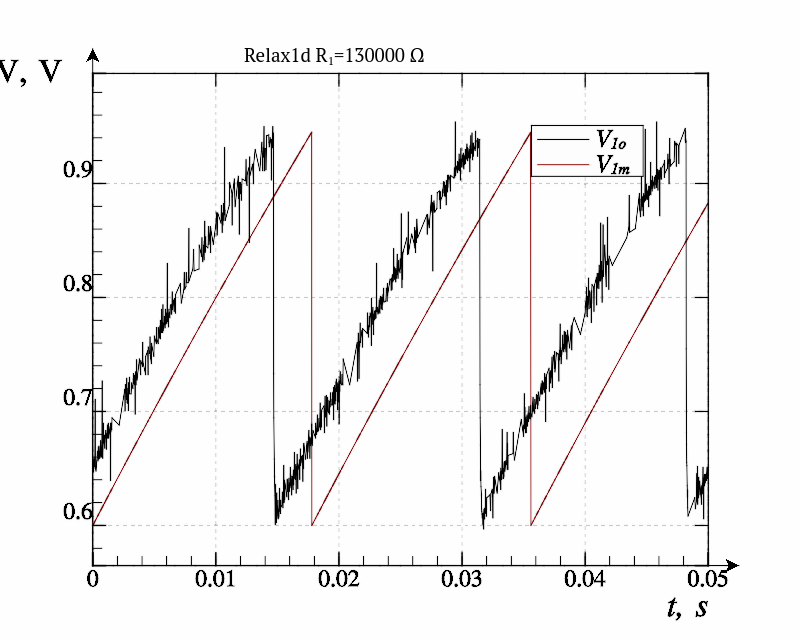
\includegraphics[width=0.6\textwidth]{p/relax1d_read_cmp-p_t_r1=130k.png} }
\caption{Залежності $V_1(t $ отримані в реальному експерименті ``relax1d'', в порівнянні результатами моделювання при $ R_1 = \SI{130}{\kilo \ohm} $}
\label{atu:f:relax1d_read_cmp-p_t_r1}
\end{figure}

Отримана форма сигналу також свідчить про те, що в цих умовах
можна використовувати як поняття частоти, так і періоду
сигналу. Вид спектрів отриманих в результаті експерименту має
набір яскраво виражених частот (рис.~\ref{atu:f:relax1d_f_r1}), при
цьому перший пік визначає частоту, і відповідно, період
сигналу. При цьому, для отримання цих значень зовсім не
обов'язково проводити досить витратний Фур'є аналіз сигналу ---
досить виміряти час, в яке вкладається досить велика кількість
періодів.

\begin{figure}[htb!]
  \centerline{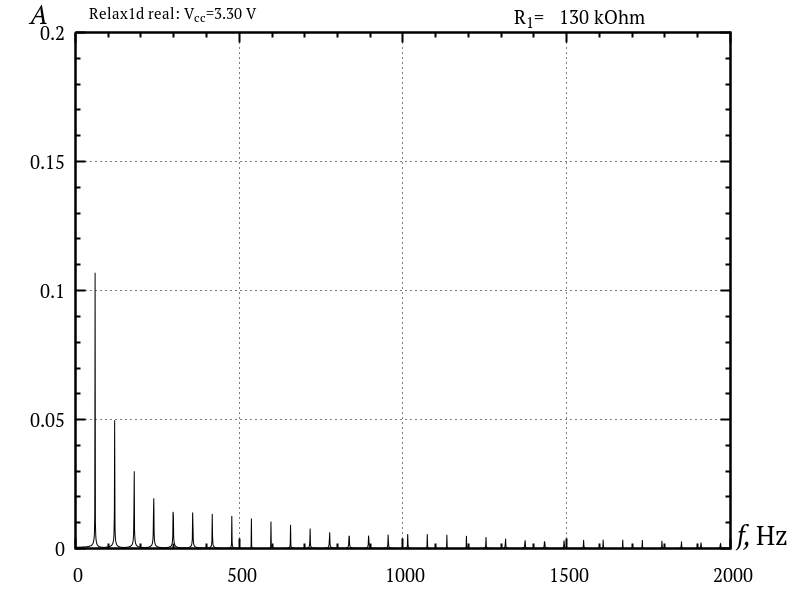
\includegraphics[width=0.6\textwidth]{p/relax1d_f_r1=130k.png} }
\caption{Спектр сигналу $ V_1 (t) $ отриманого в реальному експерименті ``relax1d'' при $ R_1 = \SI{130}{\kilo \ohm} $}
  \label{atu:f:relax1d_f_r1}
\end{figure}

При цьому з'являється можливість порівняння періодів не тільки
експериментальних і модельних результатів, але і отриманих
теоретично (\ref{atu:eq:T_u_relax}) при досить жорстких обмеженнях.


\begin{figure}[htb!]
  \centerline{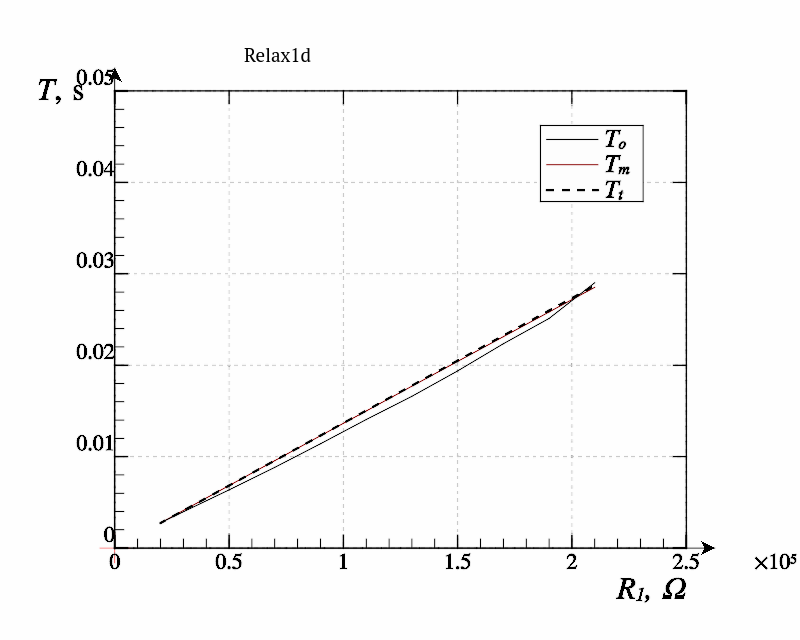
\includegraphics[width=0.6\textwidth]{p/relax1d_read_cmp-p_R1_T.png} }
\caption{Залежності $ T (R_1) $ в реальному експерименті ``relax1d'', отриманої в результаті моделювання, і теоретичні (\ref{atu:eq:T_u_relax})}
\label{atu:f:relax1d_read_cmp-p_R1_T}
\end{figure}

% TODO: more R_1: measure again

Як видно з графіків, (рис.~\ref{atu:f:relax1d_read_cmp-p_R1_T}) результати
чисельного моделювання практично повністю збігаються з
теоретично передбаченими. Відмінність від експерименту при
цьому не перевищує 5\%, що досить непогано, враховуючи безліч
неврахованих в моделі факторів. Таким чином, для одного
генератора модель дає хороший збіг з експериментом, і може
використовуватися для подальших досліджень.

При зростанні
$ R_1 $ до величини порядку
$ \SI{420}{\kilo \ohm} $ спостерігався зрив генерації і перехід в
режим стабілізації. Екстраполюючи отримані результати, можна
очікувати, що в системі з трьома такими генераторами аналогічні
явища повинні спостерігатися при
$ R_b \approx \SI{100}{\kilo \ohm} $.

При використанні в якості елемента, що перемикає, одного
генератора тригера Шмідта (позначимо як ``relax1ds''), були отримані
аналогічні результати, але з певними відмінностями. Форма
коливань має менш лінійний вид, що обумовлено дещо більшим
значенням безрозмірною величини
$ v \Tidx{on} \approx 0.3 $.

\begin{figure}[htb!]
  \centerline{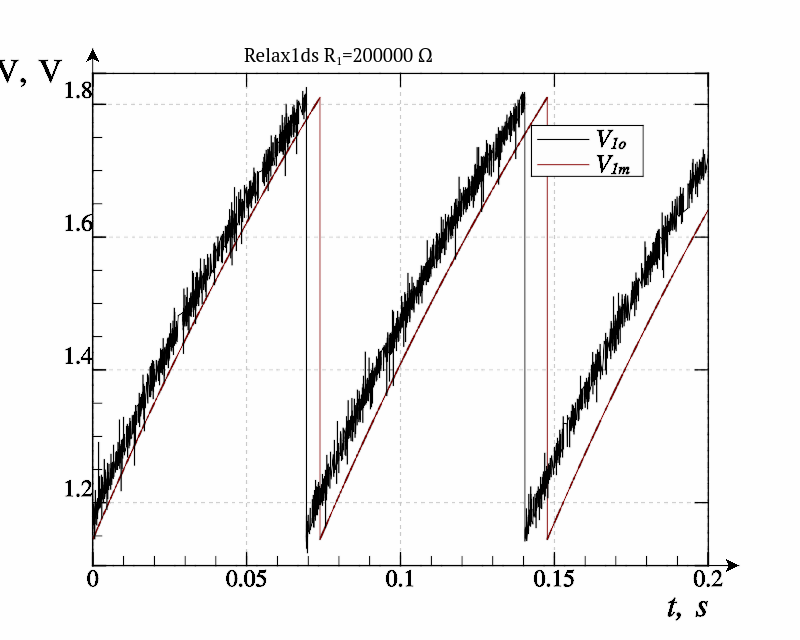
\includegraphics[width=0.6\textwidth]{p/relax1ds_read_cmp-p_t_r1=200k.png} }
\caption{Залежності $ V_1 (t) $ отримані в реальному експерименті ``relax1ds'', в порівнянні результатами моделювання при $ R_1 = \SI{200}{\kilo \ohm} $}
\label{atu:f:relax1ds_read_cmp-p_t_r1}
\end{figure}

Спектр сигналу
$V_1(t) $ має абсолютно аналогічний вид (рис.~\ref{atu:f:relax1ds_f_r1}), за
винятком того, що через більшу величину доступного значення
$R_1$, а отже, меншу частоту, відносна роздільна здатність
чисельного перетворення Фур'є виявилася менше, ніж в
попередньому випадку. Проте вигляд спектра дозволяє визначити
і виміряти період.

\begin{figure}[htb!]
  \centerline{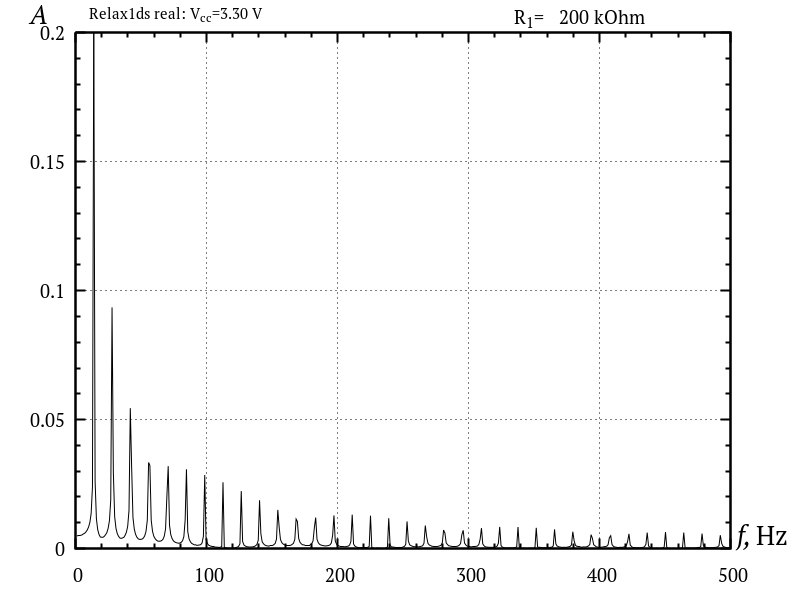
\includegraphics[width=0.6\textwidth]{p/relax1ds_f_200000.png} }
\caption{Спектр сигналу $ V_1 (t) $ отриманого в реальному експерименті ``relax1ds'' при $ R_1 = \SI{200}{\kilo \ohm} $}
  \label{atu:f:relax1ds_f_r1}
\end{figure}

Істотною відмінністю даного генератора від схеми з двома
біполярними транзисторами є той факт, що не відбувається зрив
генерації при істотному зростанні
$R_1$. В експериментах генерація спостерігалася навіть при
$ R_1 = \SI{9}{\mega \ohm} $, що практично не відрізняється від вхідного
опору вимірювальних ланцюгів. Тому, наступний графік
представлений для істотно більшого діапазону величини
$R_1$.

Залежності експериментального, модельного і теоретичного періодів
від величини
$ R_1 $ представлені на рис.~\ref{atu:f:relax1ds_read_cmp-p_R1_T}.


\begin{figure}[htb!]
  \centerline{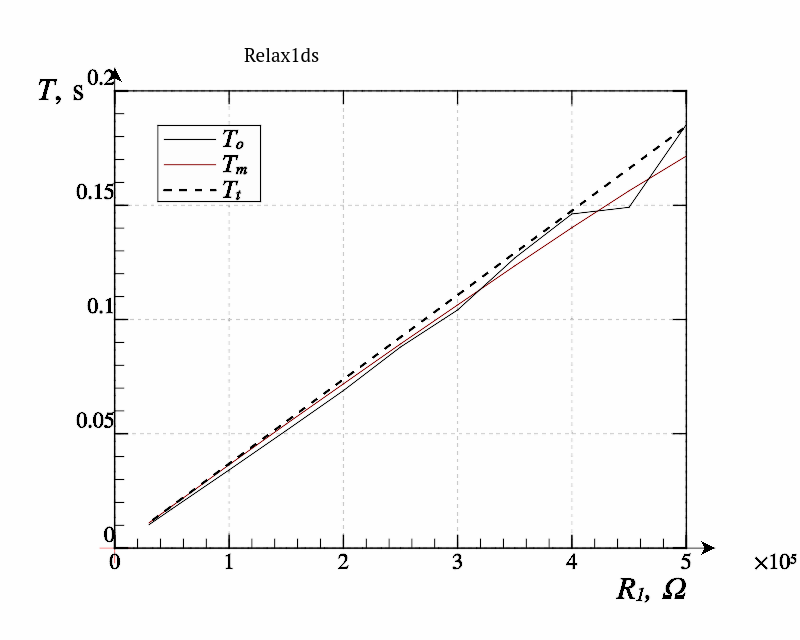
\includegraphics[width=0.6\textwidth]{p/relax1ds_read_cmp-p_R1_T.png} }
\caption{Залежності $ T (R_1) $ в реальному експерименті ``relax1ds'', отриманої в результаті моделювання, і теоретичні (\ref{atu:eq:T_u_relax})}
\label{atu:f:relax1ds_read_cmp-p_R1_T}
\end{figure}

За винятком однієї точки, різниця між експериментальними
і модельними значеннями менше, ніж для системи ``relax1d''. При
цьому спостерігається мала, але все ж помітна розбіжність між
теоретичними і модельними значеннями. В першу чергу, це пов'язано
з тим, що модель, крім явищ, описаних в теоретичному наближенні,
враховує також струми витоку, що стає більш помітним при
зростанні $R_1$.

Аналогічним способом порівняти результати експериментів
і чисельного моделювання для системи з трьох пов'язаних
генераторів не представляється можливим. Навіть для
складно-періодичного режиму візуальне порівняння форми
коливань не має сенсу, а складні спектри не дають можливості
отримати і порівняти залежності частоти від будь-якого
параметра. Практично єдиним виходом є використання критеріїв
ідентифікації, які будуть розглянуті далі. Проте, як грубої
попередньої перевірки адекватності може служити знову ж
порівняти той залежності форми аттракторов від параметра, а
також характерні особливості спектрів.

Розглянемо і порівняємо форми аттракторов для об'єкта ``relax3d''
і його моделі в разі слабо-пов'язаного режиму, при
$ R_b = \SI{10}{\kilo \ohm} $ (рис.~\ref{atu:f:relax3d_mo_v1v2v3m_03})

\begin{figure}[htb!]
  \centerline{
    \hfill
    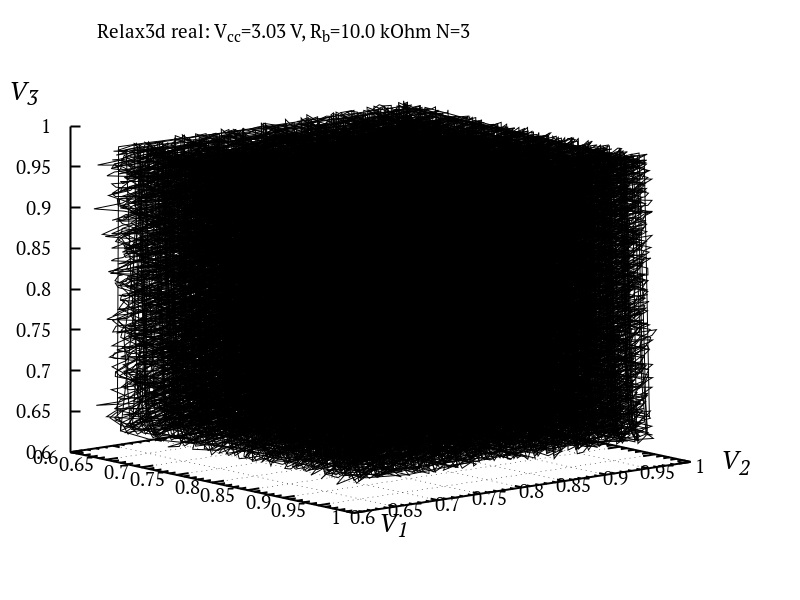
\includegraphics[width=0.48\textwidth]{p/relax3_v1v2v3_03.png}
    \hfill
    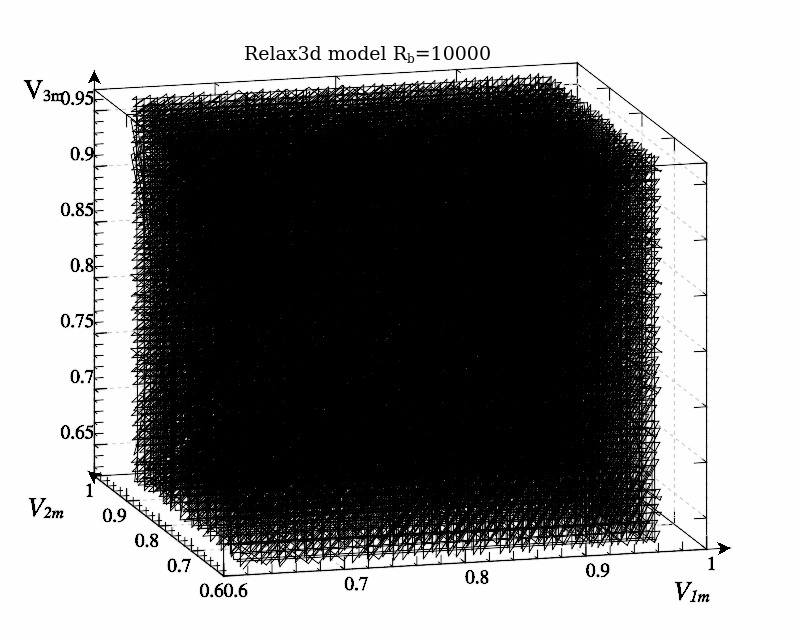
\includegraphics[width=0.48\textwidth]{p/relax3d_read_q-p_v1v2v3m_03a.png}
    \hfill
  }
\caption{Аттрактори, отримані для об'єкта і моделі при $ R_b = \SI{10}{\kilo \ohm} $}
\label{atu:f:relax3d_mo_v1v2v3m_03}
\end{figure}

Форми аттракторов в обох випадках мають однакову щільно
заповнену форму. І у моделі, і у об'єкту генератори працюють
практично незалежно, сигнали мають лінійчатих спектри
(рис.~\ref{atu:f:relax3d_mo_f_03}), але більш складні, ніж у незалежних
генераторів. Практично, це перевірка режиму, близького до
незалежних генераторів, і результати моделювання досить повно
відображають цей факт.


\begin{figure}[htb!]
  \centerline{
    \hfill
    \includegraphics[width=0.48\textwidth]{p/relax3_f_03.png}
    \hfill
    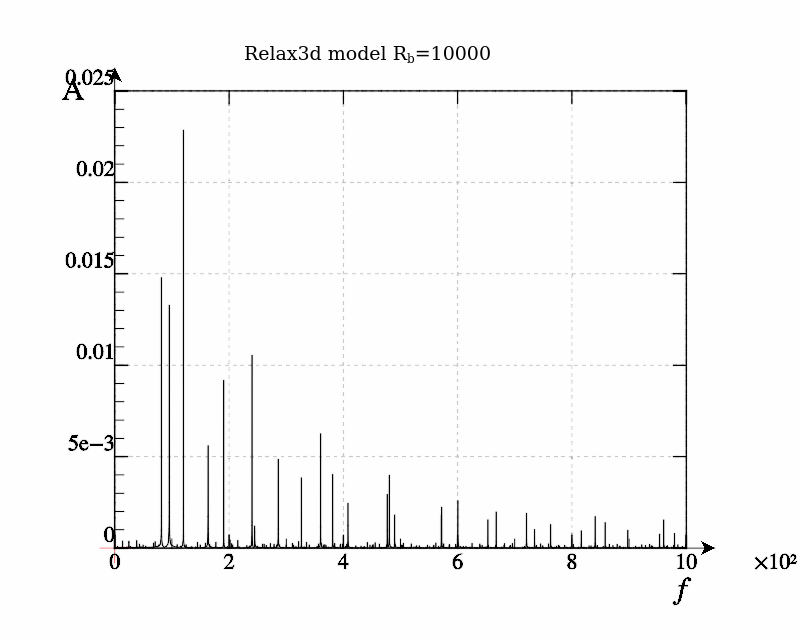
\includegraphics[width=0.48\textwidth]{p/relax3d_read_q-p_fm_03a.png}
    \hfill
  }
\caption{Спектри сигналу $ V_b (t) $ об'єкта і моделі при $ R_b = \SI{10}{\kilo \ohm} $}
\label{atu:f:relax3d_mo_f_03}
\end{figure}

Для хаотичного режиму для аттракторов спостерігається тільки
якісна схожість (рис.~\ref{atu:f:relax3d_mo_v1v2v3m_17}). При подальшому
зростанні значення параметра як у моделі, так і у об'єкту
спостерігається вироджена поведінка.


\begin{figure}[htb!]
  \centerline{
    \hfill
    \includegraphics[width=0.48\textwidth]{p/relax3_v1v2v3_17.png}
    \hfill
    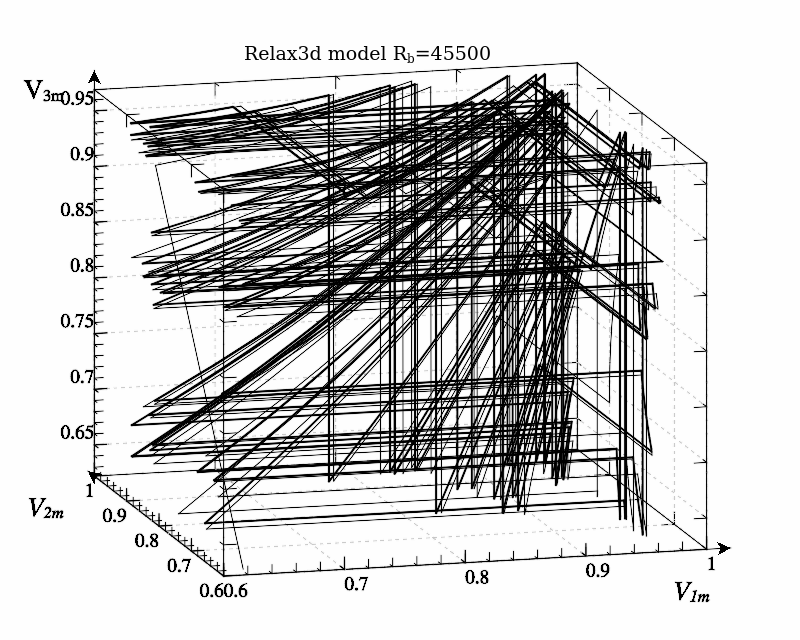
\includegraphics[width=0.48\textwidth]{p/relax3d_read_q-p_v1v2v3m_17a.png}
    \hfill
  }
\caption{Аттрактори, отримані для об'єкта і моделі при $ R_b = \SI{45.5}{\kilo \ohm} $}
  \label{atu:f:relax3d_mo_v1v2v3m_17}
\end{figure}


Спектри моделі і об'єкта в цьому режимі досить схожі саме через
свою суцільність і нерегулярність (рис.~\ref{atu:f:relax3d_mo_f_17}). Виділити
якусь домінуючу частоту не представляється можливим, хоча
певні піки на тлі суцільного спектра цілком помітні.

\begin{figure}[htb!]
  \centerline{
    \hfill
    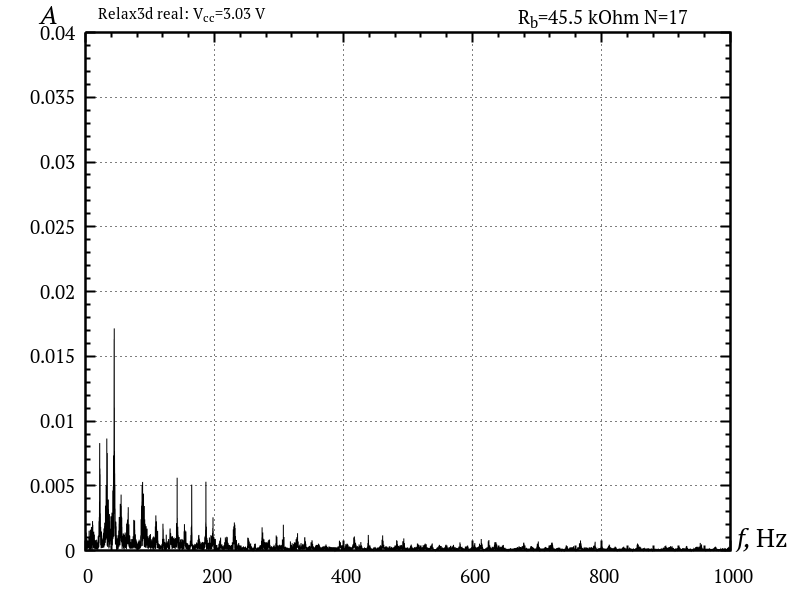
\includegraphics[width=0.48\textwidth]{p/relax3_f_17.png}
    \hfill
    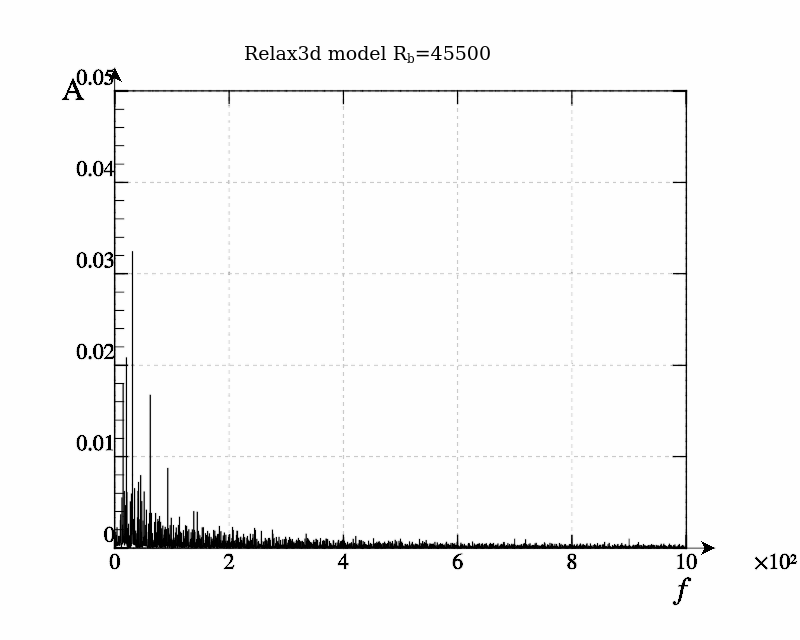
\includegraphics[width=0.48\textwidth]{p/relax3d_read_q-p_fm_17a.png}
    \hfill
  }
\caption{Спектри сигналу $ V_b (t) $ об'єкта і моделі при $ R_b = \SI{45.5}{\kilo \ohm} $}
\label{atu:f:relax3d_mo_f_17}
\end{figure}

Також слід зазначити, що незважаючи на схожість аттракторов
і спектрів об'єкта і моделі при певних значеннях параметра,
моменти перемикання між режимами, і сама кількість таких
перемикань дотримуються дуже приблизно. Така поведінка
характерна для систем хаотичної динаміки, коли не тільки
малі зміни в параметрах або початкових умовах приводять до
разбіганню траєкторій, а й зазвичай малі відмінності в
структурі моделі призводять до аналогічного результату.



\section{Критерії ідентифікації систем з трьох пов'язаних релаксаційних генераторів}

Розглянемо можливі критерії для системи релаксаційних
генераторів. В першу чергу має сенс розглянути критерії,
засновані на фізичних принципах. Як вже було зазначено,
використання в якості критерію періоду коливань не
має сенсу навіть в разі складно-періодичного режиму, не
кажучи вже про хаотичний.

Безпосереднє застосування енергетичних критеріїв для систем
такого типу також не цілком обґрунтоване --- в системі таке
співвідношення між можливостями джерела енергії та споживачами
(релаксаційним елементами), що споживання енергії лімітується
саме споживачами. При цьому моменти перемикання визначаються
відповідними рівнями потенціалів, отже, в першу чергу варто
розглядати інтегральні величини, швидше за все --- будь-яким
способом усереднені значення
$ V_b $,
$ V_1 $,
$ V_2 $,
$ V_3 $.

Розглянемо перший з кандидатів в критерії:
\begin{equation}
  q_{sv} = \overline{V_1+V_2+V_3} .
  \label{atu:eq:q_sv_relax}
\end{equation}


Як вже було зазначено (\ref{atu:eq:av_lin_relax}, \ref{atu:eq:T_u_lin_relax}) ці величини
безпосередньо пов'язані з нелінійністю залежностей
$ V_i (t) $, і залежність досить слабка. При цьому слід зазначити
досить несподіваний факт --- при збільшенні
$ R_b $, а отже погіршенні можливостей джерела живлення, середня
напруга на релаксаційних елементах росте~(рис.~\ref{atu:f:relax3d_q},
\ref{atu:f:relax3ds_q}). Це пояснюється тим, що при зростанні
$ R_b $ генератори все більшу частку часу витрачають на очікування
перед спрацюванням  елемента, що перемикає.

Таким чином, величину
$q_{sv}$ можна використовувати в якості критерію, але малий
діапазон її змін, укупі з похибками вимірювання, перешкоджає
створенню ефективної системи ідентифікації на цієї основі.


Наступна величина, яку має сенс використовувати в якості
критерію,
%
\begin{equation}
  q_{vb} = \overline{V_b} .
  \label{atu:eq:q_vb_relax}
\end{equation}
%
має безпосередній зв'язок з ідентифікованим параметром
$ R_b $, і, на перший погляд, повинна краще підходити для створення
системи ідентифікації. Проте, аналіз як реальних, так і модельних
залежностей~(рис.~\ref{atu:f:relax3d_q}, \ref{atu:f:relax3ds_q}), показує, що даний
критерій має переваги при малих значеннях
$ R_b $, при яких зв'язок між релаксаційним елементами мінімально, і
хаотична поведінка не спостерігається. На перший погляд,
це може бути пов'язано про зворотною залежністю
$ q_{vb} (R_b) $, і застосування критерію виду
%
\begin{equation}
  q_{hv} = \frac{1}{\overline{V_b}} .
  \label{atu:eq:q_hb_relax}
\end{equation}
%
може виправити ситуацію. Проте, як результати моделювання,
так і натурний експеримент показують, що це не так. Нелінійна
залежність середнього струму через елемент від середнього
падіння напруги не дає можливості ефективно використовувати критерій
$q_{hv}$.

Розглянемо комбінований критерій
%
\begin{equation}
  q_{rv} = \frac{\overline{V_1+V_2+V_3}}{\overline{V_b}}.
  \label{atu:eq:q_rv_relax}
\end{equation}


Аналіз отриманих залежностей~(рис.~\ref{atu:f:relax3d_q}, \ref{atu:f:relax3ds_q})
дає підстави вважати, що цей критерій --- кращий серед
розглянутих. Більш того, він є безрозмірним, що є важливою
властивістю критерію --- швидше за все, при зміні параметрів
системи параметри системи ідентифікації не
доведеться переналаштовувати.

\begin{figure}[htb!]
  \centerline{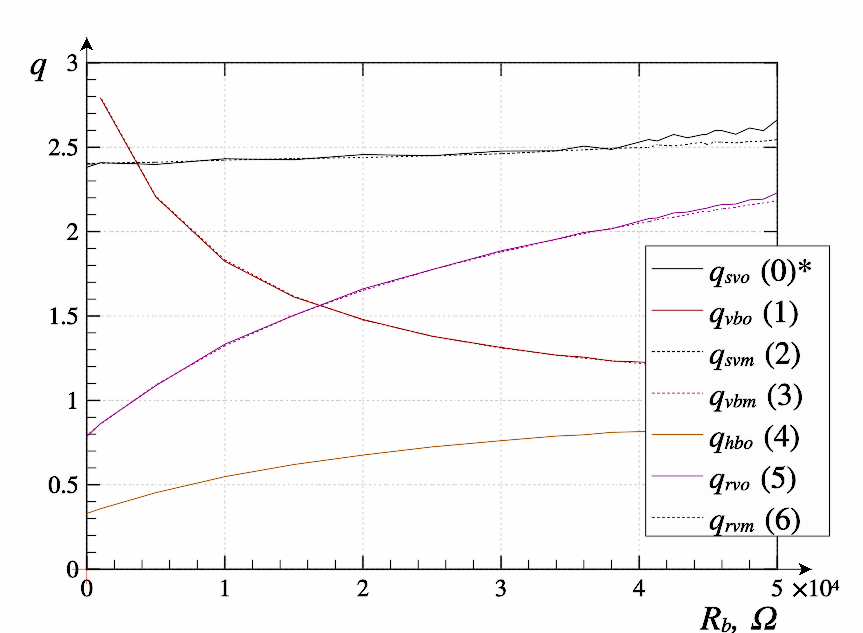
\includegraphics[width=0.7\textwidth]{p/relax3d_read_q-p_q1.png} }
  \caption{Залежності для розглянутих критеріїв ідентифікації для системи релаксаційних генераторів на парі компліментарних транзисторів}
  \label{atu:f:relax3d_q}
\end{figure}

\begin{figure}[htb!]
  \centerline{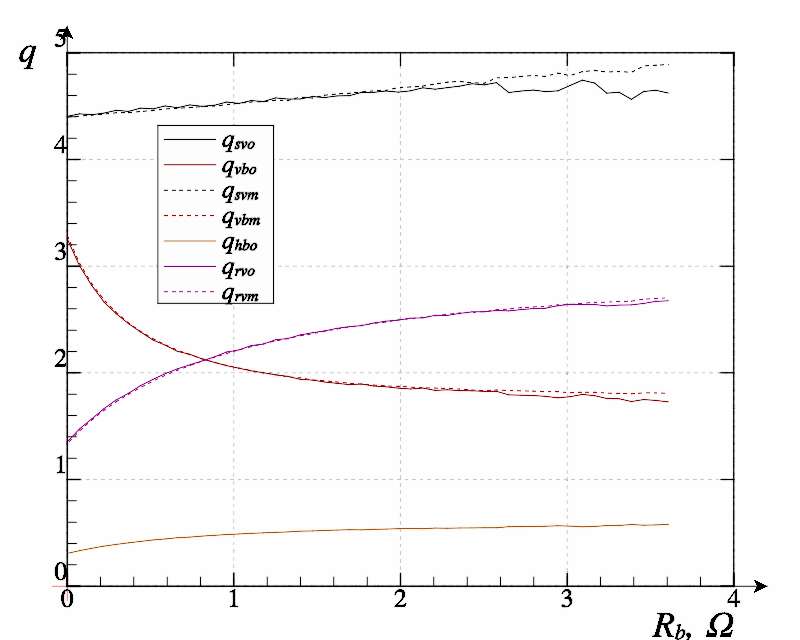
\includegraphics[width=0.7\textwidth]{p/relax3ds_read_q-p_q1.png} }
\caption{Залежності для розглянутих критеріїв ідентифікації для системи релаксаційних генераторів на тригерах Шмідта}
  \label{atu:f:relax3ds_q}
\end{figure}

На представлених графіках наведено залежності розглянутих
критеріїв як для реальних фізичних експериментів (суцільні
лінії), так і отримані в результаті чисельного моделювання
(штрихові лінії). Близькість відповідних кривих свідчить про
достатню адекватність застосовуваних моделей. Найбільші
відмінності спостерігаються в правій частині графіків,
де істотними явищами є струми витоку, що мають нелінійну
залежність від різниці потенціалів. У цих місцях прогнозується
зростання систематичної похибки ідентифікації. Проте, не
дивлячись на ці недоліки, загальний вигляд цих залежностей
дає все підстави припускати можливість побудови працездатної
системи ідентифікації.


\section{Ідентифікація параметра системи з трьох пов'язаних релаксаційних генераторів}

Для перевірки працездатності і аналізу характеристик
пропонованих систем ідентифікації були зібрані відповідні
схеми.

Для забезпечення нестаціонарності параметра
$R_b$ в якості додаткового опору, підключеного до шини живлення
через роз'єми P7~(рис.~\ref{atu:f:relax3d_schem}) і P5~(рис.~\ref{atu:f:relax3ds_schem} )
використовувався цифровий керований потенціометр CAT5171. Даний
електронний компонент являє собою керовану по протоколу
I2C збірку резисторів. Забезпечується 256 значень керованого
опору, причому, згідно з документацією, гарантується достатня
інтегральна і диференціальна лінійність залежності опору від
переданого коду:відповідно 2 і 1 молодших розрядів. Температурна
стабільність становить 100~ppm/${}\SI{}{\celsius} $.
З недоліків слід зазначити значний розкид повного
опору щодо номіналу (20~\%). У дослідних завданнях цей недолік
нівелюється попереднім калібруванням. Час встановлення після
передачі необхідного значення становить близько
$\SI{20}{\micro \second} $, що перевищує час передачі. У свою чергу, для
даної задачі необхідний час перемикання --- від сотні
мілісекунд до одиниць секунд.

Для управління цифровим потенціометром в програмі
мікроконтролера була виділена окрема задача FreeRTOS. Для цього
завдання задавалося мінімальне і максимальне значення коду
опору, і необхідний час перемикання в мілісекундах. Витрати часу,
необхідні для власне перемикання, компенсувалися на кожній
ітерації. Основна задача, що забезпечує отримання відліків з
АЦП, синхронізувала початок своєї роботи з моментом перемикання
цифрового потенціометра. Аналіз часових витрат, як і подальша
робота системи, показали, що ресурсів мікропроцесора досить
(з урахуванням використання DMA) для виконання як зазначених
завдань, так і службових. Під час запису результатів задача,
яка керувала цифровим потенціометром, зупинялася.

З урахуванням результатів попередніх досліджень, для кожної з
розглянутої схемної реалізації було обрано діапазони зміни
опору таким чином, що б з одного боку, досить повно покрити
робочий діапазон зміни параметра. З іншого --- для того, що б при
перемиканні були реалізовані різні режими роботи генератора.

В якості методів ідентифікації для обох систем була обрана група
``Fq3zlovnAAF''. Таким чином досліджувалися різні способи оцінювання
екстремуму при одній і тій же динаміці агентів ансамблю. На
кожному з малюнків, які ілюструють процес ідентифікації, лівий
графік показує динаміку агентів, а правий --- отримані значення
ідентифікованого параметра для різних способів:$ p_{ge} $,
$ p_{le} $,
$ p_{qe} $. При моделюванні процесу ідентифікації в програмі ``qontrol''
(рис.~\ref{atu:f:relax3d_id_qontrol}) в якості даних з об'єкта використовувалися
реальні дані, записані в файли, які служили джерелом даних.

\begin{figure}[htb!]
  \centerline{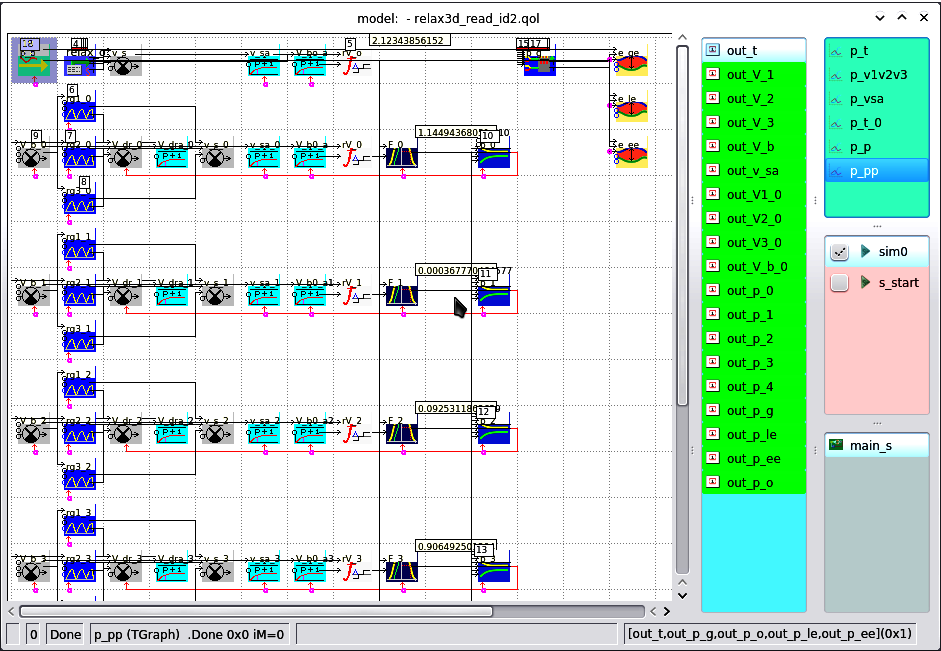
\includegraphics[width=0.9\textwidth]{p/relax3d_id_qontrol.png} }
\caption{Модель системи ідентифікації для генератора ``relax3d'' в програмі ``qontrol'' з використанням даних фізичного експерименту}
\label{atu:f:relax3d_id_qontrol}
\end{figure}

Для системи ``relax3d'' представлені результати трьох експериментів,
кожен з яких полягав в отриманні даних (відліків
$ V_b (t) $,
$ V_1 (t) $,
$ V_2 (t) $,
$ V_3 (t) $) з реального генератора, з подальшим моделюванням процесу
ідентифікації в програмі ``qontrol ''.

Параметри першого експерименту для системи ``relax3d'':
%
\begin{equation}
  \begin{array}{c}
    R_{b,\min} = \SI{30.0}{\kilo\ohm};
    \;
    R_{b,\max} = \SI{45.0}{\kilo\ohm};
    \;
    T_{R_b} = \SI{1.000}{\second};
  \\
    R_b(t) = \SI{37.5}{\kilo\ohm} + \SI{7.5}{\kilo\ohm} \cdot \sin( \pi ( t + 5.47 ) ).
  \end{array}
  \label{atu:eq:relax3d_test1_cond}
\end{equation}

\begin{figure}[htb!]
  \centerline{
    \includegraphics[width=0.48\textwidth]{p/relax3d_read_id2-p_p_00.png}
    \hfill
    \includegraphics[width=0.48\textwidth]{p/relax3d_read_id2-p_pp_00.png}
  }
  \caption{Процес ідентифікації системи ``relax3d '' за умов \ref{atu:eq:relax3d_test1_cond} (перший експеримент)}
  \label{atu:f:relax3d_id_1}
\end{figure}

Результати моделювання процесу ідентифікації в першому
експерименті~(рис.~\ref{atu:f:relax3d_id_1}) показують, що запропонована
система ідентифікації виявилася працездатною. При цьому
слід зазначити, що в першому експерименті використовувалася
максимальна амплітуда зміни параметра, отже основний внесок
вносять ``крайні'' агенти, найбільш схильні до впливу границь
робочої області, проте, були отримані цілком задовільні
результати. Візуально найкращі результати були отримані при
використанні
$p_{ge} $ і
$p_{le} $, при використанні яких були отримані практично збігаються
результати. Використання
$p_{qe} $ приводить більшою статичної похибку ідентифікації на
верхній межі. Проте, середні відносні похибки ідентифікації
досить близькі. Більш того, ця похибку мінімальна саме при
використанні $ p_{qe} $.



Параметри другого експерименту для системи ``relax3d'':
%
\begin{equation}
  \begin{array}{c}
    R_{b,\min} = \SI{30.0}{\kilo\ohm};
    \;
    R_{b,\max} = \SI{42.0}{\kilo\ohm};
    \;
    T_{R_b} = \SI{1.000}{\second};
  \\
    R_b(t) = \SI{36.0}{\kilo\ohm} + \SI{6.0}{\kilo\ohm} \cdot \sin( \pi ( t + 1.33 ) ).
  \end{array}
  \label{atu:eq:relax3d_test2_cond}
\end{equation}

\begin{figure}[htb!]
  \centerline{
    \includegraphics[width=0.48\textwidth]{p/relax3d_read_id2-p_p_01.png}
    \hfill
    \includegraphics[width=0.48\textwidth]{p/relax3d_read_id2-p_pp_01.png}
  }
\caption{Процес ідентифікації системи ``relax3d'' за умов \ref{atu:eq:relax3d_test2_cond} (другий експеримент)}
\label{atu:f:relax3d_id_2}
\end{figure}

Другий експеримент відрізняється меншою амплітудою зміни
параметра. При цьому в цілому були отримані трохи гірші
результати~(рис.~\ref{atu:f:relax3d_id_2}), ніж в попередньому експерименті,
що проявилися в помітній статичної похибку ідентифікації як на
верхньому, так і на нижньому межах. Це дещо дивно, якщо врахувати
той факт, що нижні межі в цих експериментах збігаються. Швидше за
все, це було пов'язано з неконтрольованими перешкодами в процесі
вимірювання. Проте, в цілому результати цілком задовільні.



Параметри третього експерименту для системи ``relax3d'':
%
\begin{equation}
  \begin{array}{c}
    R_{b,\min} = \SI{30.0}{\kilo\ohm};
    \;
    R_{b,\max} = \SI{40.0}{\kilo\ohm};
    \;
    T_{R_b} = \SI{1.000}{\second};
  \\
    R_b(t) = \SI{35.0}{\kilo\ohm} + \SI{5.0}{\kilo\ohm} \cdot \sin( \pi ( t + 4.33 ) ).
  \end{array}
  \label{atu:eq:relax3d_test3_cond}
\end{equation}

\begin{figure}[htb!]
  \centerline{
    \includegraphics[width=0.48\textwidth]{p/relax3d_read_id2-p_p_02.png}
    \hfill
    \includegraphics[width=0.48\textwidth]{p/relax3d_read_id2-p_pp_02.png}
  }
\caption{Процес ідентифікації системи ``relax3d'' за умов \ref{atu:eq:relax3d_test3_cond} (третій експеримент)}
\label{atu:f:relax3d_id_3}
\end{figure}

Третій експеримент характеризувався мінімальної амплітудою
зміни параметра, і продемонстрував візуально кращі
результати~(рис.~\ref{atu:f:relax3d_id_3}). Великі чисельні значення
відносної похибки викликані саме меншою амплітудою зміни
параметра, тобто абсолютна похибка нормувалося на меншу
величину.




Для системи ``relax3ds'' представлені результати чотирьох
експериментів, проведених в аналогічних умовах.

Параметри першого експерименту для системи ``relax3ds'':
%
\begin{equation}
  \begin{array}{c}
    R_{b,\min} = \SI{5.15}{\kilo\ohm};
    \;
    R_{b,\max} = \SI{24.84}{\kilo\ohm};
    \;
    T_{R_b} = \SI{1.000}{\second};
  \\
    R_b(t) = \SI{15.00}{\kilo\ohm} + \SI{9.84}{\kilo\ohm} \cdot \sin( \pi ( t + 1 ) ).
  \end{array}
  \label{atu:eq:relax3ds_test1_cond}
\end{equation}


\begin{figure}[htb!]
  \centerline{
    \includegraphics[width=0.48\textwidth]{p/relax3ds_read_id2_0-p_p.png}
    \hfill
    \includegraphics[width=0.48\textwidth]{p/relax3ds_read_id2_0-p_pp.png}
  }
\caption{Процес ідентифікації системи ``relax3ds'' за умов \ref{atu:eq:relax3ds_test1_cond} (перший експеримент)}
  \label{atu:f:relax3ds_id_0}
\end{figure}

Умови цього експерименту були обрані так, що б перевірити
працездатність на близькій до максимальної амплітуди зміни
параметра. Результати моделювання показують~(рис.~\ref{atu:f:relax3ds_id_0}),
що всі три підходи до визначення
$ p_e $ дозволяють в цих умовах отримати працездатну систему
ідентифікації. Час реакції на перемикання становить 0.3--0.4~s. При
цьому виявляється відмінність методів на верхньому і нижньому
межах: $p_{ge} $і
$ p_{le} $ забезпечують максимальну точність ідентифікації на нижній межі, а
$ p_{qe} $ --- на верхньому. Сумарно похибки ідентифікації для всіх трьох методів практично ідентичні.


Параметри другого експерименту для системи ``relax3ds'':
%
\begin{equation}
  \begin{array}{c}
    R_{b,\min} = \SI{9.94}{\kilo\ohm};
    \;
    R_{b,\max} = \SI{23.00}{\kilo\ohm};
    \;
    T_{R_b} = \SI{1.000}{\second};
  \\
    R_b(t) = \SI{16.47}{\kilo\ohm} + \SI{6.53}{\kilo\ohm} \cdot \sin( \pi ( t + 1 ) ).
  \end{array}
  \label{atu:eq:relax3ds_test2_cond}
\end{equation}

\begin{figure}[htb!]
  \centerline{
    \includegraphics[width=0.48\textwidth]{p/relax3ds_read_id2_1-p_p.png}
    \hfill
    \includegraphics[width=0.48\textwidth]{p/relax3ds_read_id2_1-p_pp.png}
  }
 \caption{Процес ідентифікації системи ``relax3ds'' за умов \ref{atu:eq:relax3ds_test2_cond} (другий експеримент)}
  \label{atu:f:relax3ds_id_1}
\end{figure}

Другий експеримент, з меншою амплітудою зміни параметра,
при збереженні працездатності, і, в цілому, трохи
меншими похибками ідентифікації, проявляє дещо іншу
картину~(рис.~\ref{atu:f:relax3ds_id_1}):верхня межа впевнено визначається
всіма методами, а нижній краще ідентифікується при використанні
$p_{qe} $.


Параметри третього експерименту для системи ``relax3ds'':
%
\begin{equation}
  \begin{array}{c}
    R_{b,\min} = \SI{13.06}{\kilo\ohm};
    \;
    R_{b,\max} = \SI{27.97}{\kilo\ohm};
    \;
    T_{R_b} = \SI{1.000}{\second};
  \\
    R_b(t) = \SI{20.51}{\kilo\ohm} + \SI{7.45}{\kilo\ohm} \cdot \sin( \pi ( t + 1 ) ).
  \end{array}
  \label{atu:eq:relax3ds_test3_cond}
\end{equation}

\begin{figure}[htb!]
  \centerline{
    \includegraphics[width=0.48\textwidth]{p/relax3ds_read_id2_2-p_p.png}
    \hfill
    \includegraphics[width=0.48\textwidth]{p/relax3ds_read_id2_2-p_pp.png}
  }
\caption{Процес ідентифікації системи ``relax3ds'' за умов \ref{atu:eq:relax3ds_test3_cond} (третій експеримент)}
  \label{atu:f:relax3ds_id_2}
\end{figure}

В даному експерименті середнє значення ідентифікованого
параметра зрушено в бік більших значень. І, як
наслідок, при ідентифікації на верхній межі похибка
максимальна~(рис.~\ref{atu:f:relax3ds_id_2}). В першу чергу, це пов'язано з
тим, що на цій ділянці чутливість критерію до зміни параметра
мінімальна. Грає свою роль і збільшення помилок при моделюванні
режиму з мінімальним енергоспоживанням. Проте, навіть в цих
умовах методи зберігають працездатність.


Параметри четвертого експерименту для системи ``relax3ds'':
%
\begin{equation}
  \begin{array}{c}
    R_{b,\min} = \SI{5.52}{\kilo\ohm};
    \;
    R_{b,\max} = \SI{18.40}{\kilo\ohm};
    \;
    T_{R_b} = \SI{1.000}{\second};
  \\
    R_b(t) = \SI{11.96}{\kilo\ohm} + \SI{6.44}{\kilo\ohm} \cdot \sin( \pi ( t + 1 ) ).
  \end{array}
  \label{atu:eq:relax3ds_test4_cond}
\end{equation}

\begin{figure}[htb!]
  \centerline{
    \includegraphics[width=0.48\textwidth]{p/relax3ds_read_id2_3-p_p.png}
    \hfill
    \includegraphics[width=0.48\textwidth]{p/relax3ds_read_id2_3-p_pp.png}
  }
\caption{Процес ідентифікації системи ``relax3ds'' за умов \ref{atu:eq:relax3ds_test4_cond}}
  \label{atu:f:relax3ds_id_3}
\end{figure}

Результати четвертого експерименти ще раз підтверджують
працездатність запропонованих методів. В цілому, в різних
експериментах різні методи показували кращі результати, проте
в цілому результати приблизно рівнозначні. Практично неможливо
в даних умовах вибрати кращий метод, з урахуванням того факту,
що значення ідентифікованого параметра заздалегідь не відомі.

Розглянемо залежності помилок ідентифікації від параметрів
самої системи ідентифікації. В першу чергу слід розглянути
вплив параметра
$a_q$, що визначає частотні характеристики фільтра значень
критерію. На рис.~\ref{atu:f:relax3ds_read_id2_prm_0-p_a_q} представлені отримані
залежності для системи ``'relax3ds' '.

\begin{figure}[htb!]
  \centerline{\includegraphics[width=0.6\textwidth]{p/relax3ds_read_id2_prm_0-p_a_q.png} }
\caption{Залежності $\overline{e}_{r *} (a_q) $ при ідентифікації системи ``relax3ds''}
  \label{atu:f:relax3ds_read_id2_prm_0-p_a_q}
\end{figure}

Порівняння отриманої залежності зі спектрами генератора
показує, що для проведення ідентифікації достатньо подавити
тільки основні частоти. Подальше повільне зростання помилок
ідентифікації пов'язане з уповільненням реакції системи на
зміну ідентифікованого параметра.

Наступний важливий параметр системи ідентифікації ---
$ q_\gamma $ визначає чутливість кожного агента. Відповідні
залежності наведені на рис.~\ref{atu:f:relax3ds_read_id2_prm_0-p_q_gamma}.


\begin{figure}[htb!]
  \centerline{\includegraphics[width=0.6\textwidth]{p/relax3ds_read_id2_prm_0-p_q_gamma.png} }
  \caption{Залежності $ \overline{e}_{r *} (q_\gamma) $ при ідентифікації системи ``relax3ds''}
  \label{atu:f:relax3ds_read_id2_prm_0-p_q_gamma}
\end{figure}

Представлені залежності абсолютно аналогічні таким для
розглянутих процесів ідентифікації. Високі значення помилок
в лівій частині графіка відповідають надмірної чутливості
функції якості, а відносно повільне зростання в правій
частині графіка --- навпаки, недостатньою. Ця недостатня
чутливість частково компенсується способом визначення величини
$ p_e $. Найкращим чином ця компенсація працює при використанні
$ p_{qe} $, а найгіршим --- при
$ p_{ge} $, коли в результаті враховується вплив практично всіх
агентів.

Вплив параметра
$ v_f $, одного з основних, що визначають динаміку пошукових
агентів, представлено на рис.~\ref{atu:f:relax3ds_read_id2_prm_0-p_v_f}.

\begin{figure}[htb!]
  \centerline{\includegraphics[width=0.6\textwidth]{p/relax3ds_read_id2_prm_0-p_v_f.png} }
  \caption{Залежності $ \overline{e}_{r *} (v_f) $ при ідентифікації системи ``relax3ds ''}
  \label{atu:f:relax3ds_read_id2_prm_0-p_v_f}
\end{figure}

Значення при
$ v_f = 0 $ відповідають нерухомим агентам. Подальше повільне
зменшення помилок ідентифікації обумовлене двома
протидіючими факторами. Перший --- зменшення похибки через
більш швидке зміщення агентів після стрибка параметра. Другий,
протилежної дії --- збільшення амплітуди блукання агентів
через порушення стійкості пошуку. Проте, кожен пошуковий агент
в методі має обмежену область переміщення, що
забезпечує стійкість методу в цілому, навіть при нестійкості
динаміки одного об'єкта.

Наступний параметр ---
$ k_e $ --- також впливає на динаміку агента, але враховується
тільки ``прагнення'' агента до передбачуваного екстремуму. Отже,
графік повинен бути схожим на попередній, що і підтверджується
результатами моделювання (рис.~\ref{atu:f:relax3ds_read_id2_prm_0-p_k_e}).

\begin{figure}[htb!]
  \centerline{\includegraphics[width=0.6\textwidth]{p/relax3ds_read_id2_prm_0-p_k_e.png} }
  \caption{Залежності $ \overline{e}_{r *} (k_e) $ при ідентифікації системи ``relax3ds''}
  \label{atu:f:relax3ds_read_id2_prm_0-p_k_e}
\end{figure}

Вплив параметра
$ k_c $ на динаміку агента має дещо іншу природу
(рис.~\ref{atu:f:relax3ds_read_id2_prm_0-p_k_c}). При малих значеннях цього параметра
рух агента в межах своєї ``смуги'' обмежується тільки взаємодією
з сусідами, що призводить до колективних зсувів агентів. Високі
значення цього параметра істотно обмежують можливість
зміщення агентів, що природно призводить до збільшення похибки
ідентифікації. Таким чином, для цього параметра існує значення,
при якому похибка ідентифікації мінімальна. При цьому,
вплив цього параметра дуже малий.

\begin{figure}[htb!]
  \centerline{\includegraphics[width=0.6\textwidth]{p/relax3ds_read_id2_prm_0-p_k_cl.png} }
  \caption{Залежності $ \overline{e}_{r *} (k_c) $ при ідентифікації системи ``relax3ds''}
  \label{atu:f:relax3ds_read_id2_prm_0-p_k_c}
\end{figure}

Залежність похибки ідентифікації від параметра
$k_n$ також має екстремальний характер, і так само слабко виражені
(рис.~\ref{atu:f:relax3ds_read_id2_prm_0-p_k_n}). Більш того, через те, що крайні
моделі мають фіксоване значення параметрів, а кількість агентів
невелика (5), цей параметр відіграє не тільки роль обмежувача
``скупченості'' агентів, але і ``допомагає'' попередньому
параметру, ``прив'язуючи'' рухливі моделі до нерухомих.


\begin{figure}[htb!]
  \centerline{\includegraphics[width=0.6\textwidth]{p/relax3ds_read_id2_prm_0-p_k_cn.png} }
  \caption{Залежності $ \overline{e}_{r *} (k_n) $ при ідентифікації системи ``relax3ds''}
  \label{atu:f:relax3ds_read_id2_prm_0-p_k_n}
\end{figure}

\section{Висновки по розділу \thechapter}

В цілому, результати експериментів, моделювання динаміки систем
пов'язаних релаксаційних генераторів і процесів ідентифікації
параметра
$ R_b $, що визначає величину зв'язку, дозволяють зробити
наступні висновки:

\begin{itemize}

  \item
    Система з трьох пов'язаних через ланцюг живлення релаксаційних
    генераторів, в залежності від величини зв'язку проміж ними,
    може проявляти як практично незалежні коливання, так і
    складно-періодичну і хаотичну динаміку.


  \item
    Вид аттракторов цієї системи в разі слабо-зв'язаних коливань, є
    досить незвичайним: практично повністю заповнений прямокутний
    паралелепіпед, а вид аттрактора в хаотичних режимах не є
    модифікацією аттракторов найбільш відомих хаотичних систем.


  \item
    Комбінований критерій ідентифікації (\ref{atu:eq:q_rv_relax}) забезпечує
    найвищу якість ідентифікації з розглянутих.

  \item
    Системи мультиагентної ідентифікації ``Fq3zlovnAAF ''
    продемонстрували на реальних тестових даних добру
    працездатність.

  \item
    Залежності питомих помилок ідентифікації від параметрів
    системи ідентифікації мають характерний для розглянутих систем
    ідентифікації вид.

  \item
    Значення параметрів
    $ v_f $,
    $ k_e $,
    $ k_c $,
    $ k_n $ можна варіювати в широкому діапазоні, без істотного
    погіршення якості ідентифікації. Це спостереження підкреслює
    адаптивні властивості ансамблевих пошукових методів.

\end{itemize}


Список використаних джерел у даному розділі наведено у повному
списку використаних джерел під номерами
\cite{horowitz},
\cite{atu_st104b},
\cite{atu_asau19},
\cite{kennedy1999},
\cite{atu_st107}.


